\documentclass[10pt,journal]{IEEEtran}
\usepackage[l2tabu,orthodox]{nag}
\usepackage[utf8x]{inputenc}
\usepackage[british]{babel}
\usepackage{ifpdf}
\ifpdf
  \usepackage[babel=true]{microtype}
\fi
\usepackage{amsmath}
\usepackage[all]{onlyamsmath}
\usepackage{newtxtext}
\usepackage{newtxmath}
\usepackage{upquote}
\usepackage{graphicx}
\usepackage{url}
\usepackage[caption=false]{subfig}
\usepackage{booktabs}
\usepackage{listings}
\usepackage{algorithm}
\usepackage{algorithmic}
\usepackage{color}

\usepackage{verbatim}
\usepackage[table]{xcolor}
\usepackage{siunitx}
\usepackage{tabularx}
\usepackage{rotating}
\usepackage{fancyvrb}
\usepackage{balance}

\newcommand{\todo}[1]{\textcolor{red}{(to do: #1)}}
\newcommand{\narrative}[1]{\textcolor{blue}{(narrative: #1)}}

\begin{document}
\title{TCP Hollywood: An Unordered, Time-Lined, TCP for Networked Multimedia Applications}
\author{
  Stephen McQuistin,
  Colin Perkins, and
  Marwan Fayed
}

\lstset{
  basicstyle=\scriptsize\ttfamily,
  language=c,
  breaklines=true,
}

\maketitle
%==================================================================================================
\section*{abstract}

Ossification of the transport-layer limits networked multimedia
applications to use TCP or UDP, despite standardisation of new transport
protocols that better support their requirements.  To improve transport for
these applications, we present TCP Hollywood, an unordered, time-lined, TCP
variant designed to support real-time multimedia traffic while being widely
deployable. Analysis of the protocol indicates that it increases the
utility of the network in lossy conditions where total one-way delay
is constrained, such as with telephony applications and low-latency video
streaming. This allows retransmissions to be useful in cases where they
are not with standard TCP, improving the timely good-put of the protocol
and reducing overheads. This analysis is validated with simulated performance
evaluations.
Initial experiments show that TCP Hollywood is deployable on the Internet,
successfully operating on all major fixed and mobile
networks in the UK, with safe failure modes.

%==================================================================================================
\section{Introduction}
\label{sec:introduction}

% !TEX root = ../utltcp-paper.tex

Real-time networked multimedia applications have long contributed to
Internet traffic. This can take the form of telephony \cite{RFC3261},
video conferencing \cite{jennings:2013:webrtc}, live or on-demand TV
and movies \cite{cha:2008:watching-tv,stockhammer:2011:dash}, or
user-generated video. These applications, and the traffic they generate,
are rapidly increasing in popularity, and now
comprise the majority of Internet traffic \cite{cisco:2013:vni-forecast}.

The nature of such real-time traffic is that it prefers predictable and bounded
latency to strict reliability, since data that arrives too late is as
bad as data that does not arrive at all. This suggests that data should
be sent in packets that can be independently decoded
\cite{clark:1990:architecture}, to allow them to be processed irrespective
of the loss or delay of other packets. However, the requirement for efficient media
compression leads to interdependence between packet contents and codecs
that operate across multiple frames.  When coupled with
challenging network environments, such as mobile wireless, that have
unreliable delivery and unpredictable latency, the requirements for
effective media transport become difficult to satisfy.

Applications access the network via the transport layer. The transport
protocol should provide services to meet the application demands,
abstracting away details of the transport process, and delivering data with an
appropriate degree of reliability and timeliness. For real-time networked
multimedia, the transport should be trusted to minimize transport-induced
delay, and should respect (partial) reliability semantics pertaining to
media importance, deadlines, and dependencies.

Message-oriented transports, such as SCTP \cite{rfc:4960} and DCCP
\cite{rfc:4340}, ought to be suitable building blocks, but their deployment
is restricted by NATs, firewalls, and other middleboxes
\cite{hatonen:2010:gateway}. This leaves real-time applications to use
UDP or TCP, neither of which is well-suited to their needs. UDP
contributes minimal latency, making it the recommended transport to meet the
strict latency bounds of real-time applications
\cite{draft-ietf-rtcweb-rtp-usage}, but provides limited support to
applications, and is commonly blocked by enterprise firewalls. TCP prefers
reliability to timeliness, and its congestion control tends to drive up
queueing delay, but is often the only transport that can pass through
middleboxes on the path. Accordingly, and despite its problems,
TCP is rapidly becoming the de facto transport for multimedia traffic.

In this paper, we engineer TCP Hollywood in response to these trends.
TCP Hollywood is an unordered and time-lined transport protocol, that is wire
compatible with standard TCP, but eliminates two sources of transport-induced
latency, and provides reliability semantics that better suit real-time
multimedia applications.  Specifically, TCP Hollywood: 1) removes
head-of-line blocking at the receiver and delivers received data to the
application immediately, irrespective of ordering; and 2) relaxes
reliability to respect time lines provided by the application, so only
data that will arrive in time is retransmitted, otherwise retransmissions
carry new data. The combination of both design elements reduces latency
and introduces message-oriented semantics, allowing TCP Hollywood to
express inter-dependencies between messages. Crucially, TCP Hollywood is
wire-compatible with TCP, and incrementally deployable on the public
Internet.

Our implementation consists of an intermediate logic layer that sits
between the application and the kernel. Extensions in the TCP stack
facilitate out-of-order delivery, and can be enabled or disabled via
socket options. Messages are delineated in the logic layer using timing
and dependency information from the application, and COBS-encoded
\cite{chesire:1997:COBS} to survive re-segmentation that may occur in the
network. We introduce the concept of inconsistent retransmissions: if the
round-trip time (RTT) estimator indicates that a message will arrive too late to be useful,
or if a message depends on a previous unsuccessfully transmitted message,
then TCP Hollywood can exploit re-transmission slots to send new data and
avoid retransmitting useless data. The semantics of TCP are maintained by
preserving the sequence numbers in retransmitted segments, whether
inconsistent or not.
We develop an analytical framework to model the value of a retransmission
against the buffering and processing time of data at the receiver-side.
Our analysis reveals a wide range of RTT values where standard TCP
retransmissions will arrive too late to be useful. We use this model to
validate TCP Hollywood, and show that it handles retransmissions correctly.

Our contributions are as follows.  After reviewing the rationale and
requirements in Section \ref{sec:background}, we design a TCP-compatible
architecture and application programming interface (API) that eliminates
transport related, but not congestion control related, delay from TCP in
Section \ref{sec:design} (this can be used with any of the existing
proposals to reduce congestion control related delay, such as active
queue management \cite{nichols:2012:codel,khademi:2014:new-aqm} or
delay-based congestion control \cite{jin:2004:fast-tcp,brakmo:1994:tcp-vegas}).
We develop an analytic framework in Section
\ref{sec:analysis} to determine the value and content of retransmitted
data. Section \ref{sec:perfeval} describes performance evaluations based on 
a simulated VoIP application, with typical cross-traffic classes. 
Experiments to demonstrate the ease of deployment of TCP Hollywood are
discussed in Section \ref{sec:deployability}. Related work and concluding
remarks are provided in Sections \ref{sec:related} and
\ref{sec:conclusions}, respectively.

This paper is an extended version of \cite{mcquistin:2016:tcp-hollywood}.
It revises and extends the material in that paper, extending the discussion 
of service requirements and APIs for real-time applications in Section
\ref{sec:background}, adding a performance evaluation in Section
\ref{sec:perfeval}, and adding an appendix discussing reproducibility of
our results.

%==================================================================================================


%==================================================================================================
\section{Design Goals and API Requirements}
\label{sec:background} % !TEX root = ../utltcp-paper.tex

We begin by considering in more detail the rationale and requirements for an
unordered and time-lined transport protocol. It is instructive first to
establish TCP as the foundation from which to build, then understand its
negative impact in the context of live and interactive media. Doing so
establishes a set of desirable {\em real-time transport services}.

% We begin by considering in more detail the requirements for the
% transport-layer API that real-time, low-latency applications need. This
% discussion uses the vocabulary established by the Transport Services (TAPS)
% working group at the IETF, allowing us to describe the
% \textit{transport services} our API must provide.
%
% Following this, we discuss the rationale for our use of TCP as the
% foundation for a protocol that provides this API. Finally, we describe the
% high-level design needed to achieve our competing goals of latency
% reduction and wire-compatibility with TCP.

%------------------------------------------------------------------------------
\subsection{TCP Compatible Design Goals}
\label{sec:background-tcp}

Our primary design goal is to improve performance over TCP \emph{for real-time
traffic}, while maintaining the possibility of deployment on the scale of TCP and
UDP. Ossification of the transport layer means this goal can \emph{only} be achieved by
using TCP or UDP as a substrate. This is a limitation that exists in the
Internet because of middleboxes that process packets based on static views of
what is a valid transport. The operation of these middleboxes places two constraints on transport
protocols~\cite{mcquistin:2015:reinterpreting}. First, only packets containing
TCP or UDP are marked as valid by middleboxes; packets containing other transport protocols
are often rejected, and some networks also reject UDP. 
Second, middleboxes may reject valid TCP packets that don't
conform to some limited subset of the TCP protocol that they understand
\cite{honda:2011:extend-tcp}. For example, packets with the
SACK (selective acknowledgement) extension might be rejected by a
middlebox that doesn't understand that extension, and expects only regular
ACK packets.
Reliability and congestion control are desirable features.
These can be implemented by applications running over UDP,
but it is difficult to do this well \cite{RFC5405}. Accordingly,
and because it's more widely accepted by middleboxes, TCP has emerged as
the protocol of choice for real-time multimedia.

% %--------------------------------------------------------------------------
% \subsection{Design Requirements}

% ---------------------------------------------------------------------------
%\subsection{Rationale for TCP Compatibility}

% However, when streams are live and interactive these features are also the
% source of non-network latency. We use an assessment of the underlying mechanisms
% to identify the design requirements.

% Ossification of the transport layer -- due to assumptions made by the numerous
% network middleboxes that believe they understand the transport -means that we
% can only achieve our first goal by using TCP or UDP as a substrate, making
% minimal wire-visible changes. We chose to extend TCP since it provides effective
% congestion control, which is complex to replicate in UDP-based protocols, and
% because UDP is often blocked by enterprise firewalls.

% ------------------------------------------------------------------------------------------------
%\subsection{Design Requirements}
Our secondary goal is to minimize the transport-induced latency on applications.
Given TCP as a necessary substrate, appropriate modifications are needed to meet
our latency goals. TCP introduces latency in part because of (i) the nature of
its congestion control dynamics, and in part by (ii) providing an ordered,
reliable, delivery model using head-of-line blocking and retransmissions. The
former can be addressed using active queue management and/or delay-based
congestion control algorithms, and has been widely studied (e.g., 
\cite{nichols:2012:codel,khademi:2014:new-aqm,brakmo:1994:tcp-vegas}). The
latter issue is more applicable to real-time traffic, and is the subject of our
work.

Figure \ref{diagram:motivation_latency} shows explicitly the impact of
head-of-line blocking. The loss of the third segment causes subsequent segments
to be buffered at the receiver while waiting for the retransmission. Only when
the delayed segment arrives can TCP deliver the in-order sequence to the
application. The impact of retransmitted segments are exacerbated when they push
subsequent segments past the time when they're useful to the
application. Such segments are effectively lost to the application, despite
having been delivered to the host on time. It is these \emph{late losses} that
TCP Hollywood seeks to minimize.

\begin{figure}[t]
 \centering
 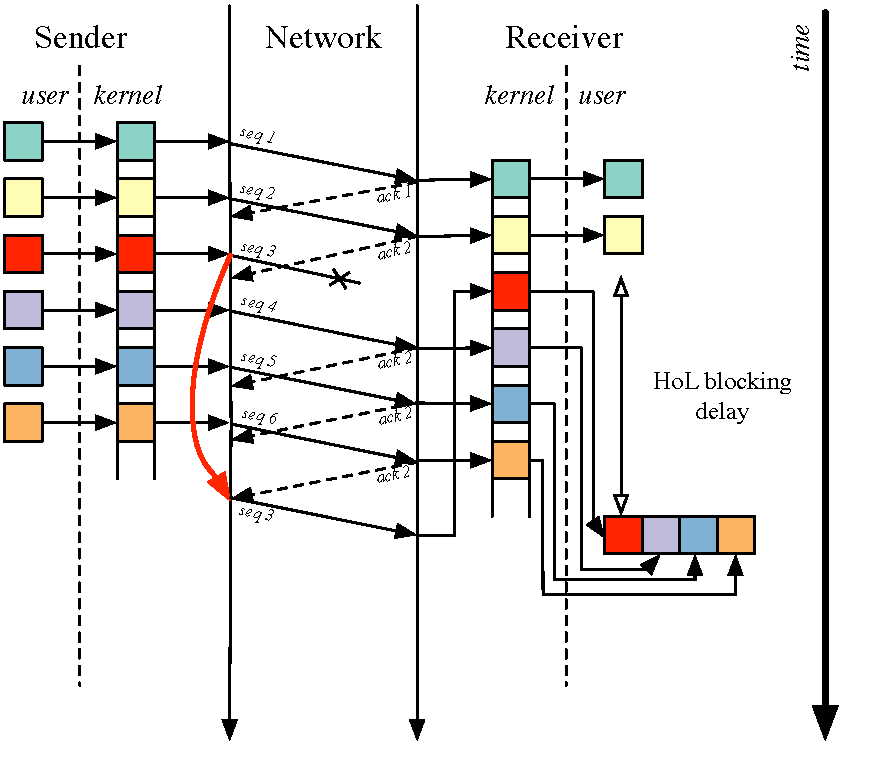
\includegraphics[scale=0.6]{figures/hol-blocking-delay.pdf}
 \caption{The interaction between head-of-line blocking and loss in TCP:
  multiple segments are delayed by a loss, and potentially delivered too late to be useful to the receiver}
\label{diagram:motivation_latency}
\end{figure}

Two requirements follow. First, to eliminate head-of-line blocking,
segments must be delivered as they arrive.  Second, retransmissions should be evaluated
against timing information to ensure delivery of useful data, by allowing
\emph{inconsistent retransmissions} to send new data in a segment that is
retransmitted. So that applications can benefit from out-of-order delivery, a
message-oriented abstraction is needed. Specifically, messages should be
independently useful to the receiver \cite{clark:1990:architecture}. The
following real-time transport services emerge as a result.




%------------------------------------------------------------------------------
\subsection{Service Requirements for Real-time Applications}

In the IETF, the Transport Services (TAPS) working group provides a vocabulary
for discussing transport protocol components~\cite{taps}. We use their
vocabulary to describe the transport services we believe are needed for
real-time multimedia. Details, as well as an abstract API, may be
found in~\cite{McQuistinANRW:2016}.

\textbf{Timing} is an implicit and salient attribute of real-time media
applications. Timing requirements determine {\em deadlines} to present media to
the application, i.e., to play audio and render video. Deadlines depend on the
nature of the application. Interactive application deadlines, such as for
telephony, video conferencing, or telepresence, range from tens to hundreds of
milliseconds. Non-interactive broadcast or on-demand streaming applications can
tolerate deadlines on the order of seconds.

Networked multimedia timing and deadline services are unusual among real-time systems. Consider that data that misses its deadline arrives too late to be usefully rendered to the user; yet that same data may be used by the application to complete a predictive decoding chain. This suggests a need to redefine the nature of reliability and ordering.

% \textbf{Timing} is a fundamental characteristic of low-latency application
% traffic, and it is foundational for our API: the other services follow from
% it. The data generated by these applications has a relative deadline
% associated with it -- the duration in which the data can be considered to
% be useful to the receiver. These relative deadlines are dependent on the
% latency requirements of the application; interactive applications (e.g.,
% telephony, video conferencing) have hard latency bounds, while
% non-interactive applications have softer bounds.

\textbf{Partial Reliability} services acknowledge that a transport might be unable to
deliver data by a given deadline. A retransmission that fails its timing
requirements leads to play-out stalls. This causes applications to block, and is
a primary cause of poor user experience. Accordingly a transport protocol
designed to meet deadlines should support partial reliability, and retransmit
only data is useful to the application.

% Supporting the timing service over a lossy, best-effort network requires
% support for \textbf{partial reliability}. There is some probability that
% packet loss will occur, and that the lost packets will have to be
% retransmitted. Since retransmissions themselves may be lost, the delay
% introduced by a fully reliable transport service is unbounded: this is
% incompatible with the timing service. Data should only be transmitted if it
% is likely to useful on reception.

\textbf{Message-oriented Dependency} services culminate from timing and partial
reliability services. Data should be transmitted to the receiver only when the
receiver can play the data in time, or when the data is needed as part of the
decoding chain. This service is further complicated because the sender should
never transmit data that relies on previous transmissions that were never
received. Managing dependencies in this fashion requires application-layer
framing~\cite{clark:1990:architecture} to provide a {\em message-oriented}
service that maintains, and transmits along, application data unit (ADU)
boundaries.

Message orientation also provides a foundation for {\em multi- or sub-stream services}. Media content can be composed of multiple streams of data, each with its own data characteristics. Audio and video, for example, may be separated into streams with different priorities, message sizes, and bitrates. Message-orientation may also be exploited in multipath environments. An independent {\em multipath service}, for example, may increase utility by scheduling packet transmissions by matching sub-path properties with sub-stream characteristics.

% A \textbf{dependency management} service is required as a result of partial
% reliability: data might depend on earlier data that was not received
% successfully, rendering it useless to the receiver. Exposing dependency
% information to the transport layer prevents such data from being sent.
%
% A partial reliability service also requires a \textbf{messaging} service to
% maximise the utility of each data packet. The application should transact
% in application data units: discrete blocks of data that are independently
% useful to the receiving application. To minimise latency, these messages
% should be delivered to the application in the order that they arrive.
%
% A \textbf{multistreaming} service is desirable. Some target
% applications comprise multiple streams (for example, distinct audio
% and video streams in a typical multimedia application). Each of these
% streams has different characteristics (e.g., message sizes, sending rates)
% that should be exposed to the transport layer.

% With metadata about different streams, a \textbf{multipath} service is
% needed to map these to different paths within the network. This mapping
% should match the characteristics of each stream with the properties of each
% network path, increase the utility of the network.

\textbf{Connections and Congestion Control} are critically important.
Networked multimedia content is increasingly encoded at variable or
adaptive bitrates, or both. Applications, user experience, and network
utilization, would be best served by the ability to respond to changes in
available bandwidth. We argue that real-time transport should rely upon,
but be agnostic to, TCP congestion control to ensure co-existence on the
wider Internet. TCP Hollywood uses TCP congestion control unchanged, and
can make immediate use of advances in TCP congestion control as they
become available.

An explicit connection-oriented service may be a lesser requirement, given
per-flow state at the endpoints is sufficient to provide 
congestion control. However, signalling messages indicating
start and end of connections can, for example, ease NAT traversal and
facilitate firewall management. Accordingly, the availability of a
connection-oriented service is desirable.

%
%  is required to protect the network, and the
% other applications that use it. The congestion control algorithm should
% account for the latency-sensitive nature of the applications. 
% Congestion control algorithms would benefit from a \textbf{connections}
% service, making use of per-connection metadata. Beyond this, having
% explicit connection setup and teardown signals may benefit in-network
% services, such as NAT traversals and firewall pinholing.
%
%
% % In the next section we present the TCP Hollywood architecture, alongside the design
% % elements that preserve TCP semantics and ensure wire-line compatibility.


% With both a message-oriented
% abstraction and timing information, the collection of message dependency
% information follows. This increases the application-awareness of the
% transport layer.


%==================================================================================================
\section{Architecture and Design}
\label{sec:design}

% !TEX root = ../utltcp-paper.tex


% Having identified the requirements in the previous section, we now present the
% overall TCP Hollywood architecture, and design of the wire protocol.

TCP Hollywood has been designed to be deployable on the ossified Internet
as it exists today, and to support partial deployments where only the sender
or the receiver has been upgraded to support the TCP Hollywood extensions.
The nature of the extensions we propose supports the former, while the
latter is achieved by splitting the functionality between a user-space
intermediary `shim' layer and a set of extensions to the kernel TCP stack.
The intermediary layer operates over either unmodified TCP, or with the
TCP Hollywood kernel extensions enabled. The user and kernel components
are represented in the overall architecture represented in Figure
\ref{diagram:architecture}. In discussing the architecture it is useful to
consider the sender separately from the receiver, and for each to consider
the user-space intermediary layer separately from the kernel TCP extensions.

\begin{figure}[t]
	\centering
	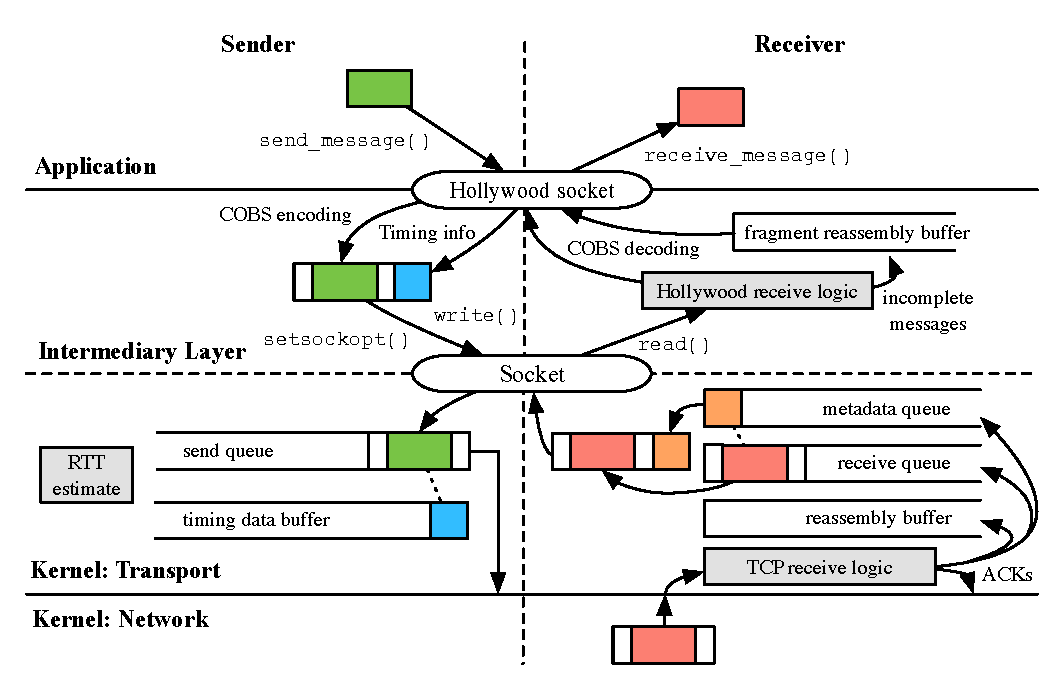
\includegraphics[width=\columnwidth,height=2.2in]{figures/message-flow-combined.pdf}
	\caption{TCP Hollywood sender and receiver architecture}
	\label{diagram:architecture}
\end{figure}

%--------------------------------------------------------------------------------------------------
\subsection{TCP Hollywood Sender architecture}
\label{subsec:sender}

The architecture of a TCP Hollywood sender is shown in the left hand side
of Figure~\ref{diagram:architecture}. The sender inherits the requirements
identified in Section~\ref{sec:background} to support a timed,
message-oriented, transport abstraction, with inconsistent retransmissions.
%This is supported by the user-space intermediary layer, and an optional
%(but highly desirable) set of changes to the in-kernel TCP sender.

The intermediary layer provides the message-oriented abstraction. It accepts
a sequence of messages (i.e., datagrams, rather than a byte stream) from the
application, with optional timeliness and dependency information,
to be delivered to the destination.
%
% For those messages that have no timeliness or dependency requirements,
%
The intermediary layer supports a sub-stream abstraction, allowing messages from multiple flows
to be multiplexed on a single transport-level connection (similar to how multiple streams
can be sent within a single SCTP association \cite{rfc:4960}).  This can
be used to cleanly multiplex audio and video flows onto a single
connection, or to distinguish multiple layers of a stream encoded using
scalable video coding~\cite{Ohm05}, for example using H.264/SVC.
%
The intermediary layer appends a sub-stream identifier to messages before
they are encoded, framed, and passed to the kernel TCP sender, with a
default sub-stream being reserved for flows where no sub-stream is
specified.  The application can provide timing or dependency data via
the intermediary layer API. This is passed to the kernel alongside the
encoded message, and used to determine whether inconsistent
retransmissions are appropriate.

To support a message-oriented abstraction over a TCP byte stream, the
TCP Hollywood flows must be resilient to re-segmentation or segment coalescing
by middleboxes. Message integrity must be protected: messages received
must have been sent, and only complete messages must be delivered.  This
is ensured by the intermediary layer, which frames messages with a leading
and trailing marker. The effect is shown in Figure~\ref{diagram:resegmentation},
where markers can be used to delineate messages irrespective of the
segmentation. The intermediary layer encodes messages with consistent overhead
byte stuffing (COBS)~\cite{CB97COBS}; this efficiently encodes the stream
to escape all zero bytes, allowing their use as framing markers, while still
providing a transparent channel that can carry any message.

The TCP sender implementation in the kernel is modified to perform
consistent segmentation, and to manage inconsistent retransmission
by tracking message timing, deadline expiration, and dependencies.
Consistent segmentation ensures that a single \texttt{write()} call made
by the intermediary layer will generate a single TCP segment, provided the
size of the segment does not exceed the MTU.
This ensures each message is sent in a separate TCP segment, allowing the
receiver to process it independently of other messages, reducing latency.
This implies disabling Nagle's algorithm (i.e., setting
the \texttt{TCP\_NODELAY} socket option) to avoid unnecessary buffering --
Nagle's algorithm would not provide a significant benefit to our target
applications, where messages are large compared to their headers.

\begin{figure}[t]
 \centering
 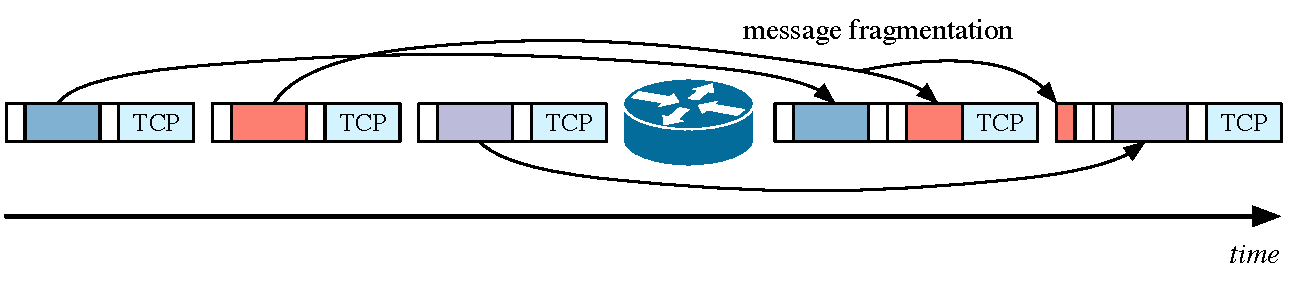
\includegraphics[width=\columnwidth,height=0.9in]{figures/message-resegmentation.pdf}
 \caption{Encoding and framing with leading and trailing markers protects
 against middlebox re-segmentation; received segments can be properly decoded}
\label{diagram:resegmentation}
\end{figure}

TCP retransmissions ensure reliability, but also inject latency that may
cause late losses. A TCP Hollywood sender has the notion of \textit{message
expiry}: a message expires when (i) RTT estimates indicate the
retransmitted message will arrive too late, or (ii) if the message depends on a
previous message that was unsuccessfully delivered. Under these circumstances
TCP Hollywood can send a new message using the same TCP sequence number space
as a previously sent message, re-writing the remaining bytes in the TCP send buffer
with new content.
To support such \emph{inconsistent retransmissions}, the intermediary layer
passes messages down to the modified kernel TCP stack along with metadata
to describe their deadline, dependency, and sub-stream. This is enabled by
calls to the Berkeley Sockets API \texttt{setsockopt()} function.
The metadata, with the exception of the sub-stream identifier, is never
transmitted on the wire, but is held locally for each message for as long
as the message is buffered (i.e., until all \texttt{ACK}s associated with
a message are received). Our kernel extensions implement a separate buffer
to hold per-message metadata.

The inconsistent retransmission logic is triggered when the standard
TCP retransmission logic would be triggered by a triple duplicate ACK
or timeout. Metadata for unacknowledged messages is then evaluated
against the current RTT estimate, to determine whether the
original message is to be retransmitted, or if an inconsistent retransmission is
to be sent, replacing the original data with new content while keeping the
same TCP sequence number. Since messages are framed and self-describing, a
receiver can decode the inconsistent retransmission.

The latency benefits of inconsistent retransmissions will be quantified in
Section~\ref{sec:analysis}.  In the interim, we emphasize the
message abstraction in this context: TCP Hollywood sends messages rather
than bytes in a data stream. Consequently, a message may be composed of
multiple fragments, split across TCP segments. To preserve the semantics at
the receiver, fragments necessary to finish a partially received message
are always retransmitted, but if no part of a message was received, it may
be replaced with a new message when its containing TCP segment
is retransmitted.

The processing overhead of TCP Hollywood at the sender is comprised of
COBS encoding at the intermediary layer, and the maintenance of metadata
in the kernel. COBS encoding requires a copy of
the message to be made, but this could be eliminated by performing the byte
stuffing as the message is being generated, as part of the multimedia
encoding. Beyond this copy, COBS is ``computationally cheap''
\cite{chesire:1997:COBS}. In the kernel, the sender maintains
metadata for each message, while the message could still be sent. Further
processing, such as estimating whether a message will arrive on time, uses
data already maintained by the kernel.

%--------------------------------------------------------------------------------------------------
\subsection{TCP Hollywood Receiver Architecture}
\label{subsec:receiver}


The receiver-side architecture of TCP Hollywood is shown on the right hand
side of Figure \ref{diagram:architecture}. Like the sender, it is composed
of a user-space intermediary layer, and TCP extensions in the kernel
receive path. The receiver supports message-oriented delivery, and
additionally eliminates head-of-line blocking. The use of inconsistent
retransmissions is invisible to the receiver.

The kernel initially processes incoming segments as would TCP. It
generates the appropriate ACKs (e.g., duplicate ACKs for out-of-order or
lost segments), and places segments into the reassembly buffer as usual.
The on-the-wire response to each received segment is \emph{identical} to
that of TCP: ACKs (and SACK blocks, or other extensions, if negotiated)
are generated in exactly the same way as standard TCP, and the congestion
response is unchanged.

Where a TCP Hollywood receiver differs from standard TCP is that all
segments, including those received out-of-order, are
delivered to the intermediary layer in the order they are received, with no
head-of-line blocking or reordering. As each segment arrives, a metadata
structure is created to store its TCP sequence number. This sequence number
is then appended to the segment as it is read by the intermediary layer.
Sequence numbers are used by the intermediary layer to delineate messages
that are encoded across multiple segments. Making segments available to the
intermediary layer as they arrive is the only change needed to the kernel
TCP code at the receiver.

The intermediary layer scans incoming segments for complete messages,
delineated by the COBS framing. If consistent segmentation was used, and
segments were not fragmented or coalesced in the network, then messages
will correspond to TCP segments. Otherwise, incomplete message fragments
are buffered in the fragment reassembly buffer awaiting missing fragments.
The relative ordering of the bytes in message fragments is established
using the TCP sequence number tag associated with received segments.
As shown in Figure \ref{diagram:architecture}, complete messages are
decoded and queued for delivery to the application. The API between
intermediary layer and application is message oriented, and includes a
message sequence number. This simplifies receiver processing compared to
the TCP stream API.

The COBS decoding process is similar to that of the receiver, incurring an
additional copy at the intermediary layer. In the kernel, our
proof-of-concept implementation maintains a metadata structure to store the
TCP sequence number and length of each incoming segment -- data that would
be otherwise lost. For incoming segments that are out-of-order, or arrive
while there are segments in the reassembly queue, we make an additional
copy (versus the TCP implementation) of the segment's payload, storing this
with the segment's metadata. While this simplifies the implementation, it
is not a requirement of the design: optimisation of our implementation
could eliminate this.

%--------------------------------------------------------------------------------------------------
\subsection{Partial Deployments and Legacy TCP Compatibility}
\label{subsec:partialdep}

The TCP Hollywood intermediary layer is a user-space library that can run
over a standard TCP implementation, using the Berkeley Sockets API, or on
a modified TCP stack using the extensions we have described. If both
sender and receiver support the kernel TCP extensions, the full
benefit described above is achieved. However, the TCP Hollywood
intermediary layer can also be deployed as part of an application,
irrespective of the state of deployment of the kernel TCP extensions.

If only the receiver supports the TCP Hollywood kernel extensions, with
a standard TCP sender, then the intermediary layer and application will
benefit from avoidance of head-of-line blocking, but not from the latency
reduction of inconsistent retransmission.
Message oriented delivery will be supported, since COBS framing is
generated by the intermediary layer at the sender, but COBS decoding may
be less efficient since messages boundaries will be less likely to be
aligned with segment boundaries.

If only the sender supports the TCP Hollywood kernel extensions, it will
generate inconsistent retransmissions, and perform consistent segmentation
as described, since both are invisible to the TCP layer of the receiver
(compatibility with middleboxes is discussed in Section~\ref{sec:deployability}).
This will improve latency, and increase efficiency of COBS decoding, at
the receiver, irrespective of whether the receiver has the TCP Hollywood
kernel extensions.

If neither sender or receiver support the TCP Hollywood kernel extensions,
the intermediary layers can communicate over a standard TCP connection. In
this case, the message oriented abstraction persists, and applications can
communicate using a TCP Hollywood socket to exchange messages, rather than
byte streams, in a congestion controlled and reliable manner, although
with no latency benefit over standard TCP.


%==================================================================================================
\section{Latency Reductions and Analysis}
\label{sec:analysis}

% !TEX root = ../utltcp-paper.tex


TCP Hollywood reduces transport latency through support of inconsistent
retransmissions, and by eliminating receiver-side head-of-line blocking. To
quantify the benefits of these two techniques to the application, we begin by
modelling the one-way transport delay, $T_\mathrm{owd}$, as:
\begin{equation}
  T_\mathrm{owd} = T_\mathrm{sender} + T_\mathrm{playout} + T_\mathrm{rtt}/2
  \label{eq:owd}
\end{equation}
where $T_\mathrm{sender}$ is the time taken for the sender to capture,
encode, and transmit a frame of media data. $T_\mathrm{playout}$ is the sum of
the de-jitter buffering delay, and the time taken to decode and render a frame
to the application at the receiver. Finally, $T_\mathrm{rtt}$ is the network
round-trip time. With no loss of generality we assume broadly symmetric network
paths in this analysis.\footnote{This assumption does not hold in ADSL and
cellular networks with asymmetric downstream and upstream links.  In these
cases, our model mis-approximates the application's upper bound on delay,
shifting the line marked ``Application Deadline'' in Figure
\ref{diagram:inconsistentretrans}. While further analysis is needed to
quantify the impact of this, it is clear that it does not change the broad
conclusion of our analysis: that TCP Hollywood increases the usable region of
retransmissions.}

The inter-frame interval of the media, i.e., the duration of media in each frame,
is denoted by $T_\mathrm{framing}$. We know that $T_\mathrm{sender} \geq
T_\mathrm{framing}$, since a frame cannot be sent before it has been captured.
Similarly at the receiver, if the media is to be decoded and rendered without
gaps, then $T_\mathrm{playout} \geq T_\mathrm{framing}$. The time needed to
encode and decode media %can generally be assumed to be
is generally negligible in comparison to the framing interval, making
$T_\mathrm{sender} \approx T_\mathrm{playout}$ a reasonable approximation in the
absence of jitter. At the receiver, however, while the media decoding and
rendering time is generally small, the de-jitter buffer duration can be
significant, and a similar approximation cannot be made.

% For a given application there will be an acceptable delay bound,
The one-way transport delay contributes to an application's acceptable delay
bound
%as set by the application %% slight mod to prevent multi-line inequality.
$T_\mathrm{max}$, such that $T_\mathrm{owd} \leq T_\mathrm{max}$. For
interactive applications, the delay bound is generally around 150ms
\cite{itu:2003:delay}, whereas streaming applications can accept longer delay
bounds (around 0.5 seconds if channel surfing is to be supported; up to tens of
seconds for on-demand streaming).

% We simplify the analysis by assuming that TCP flows
% are steady-state and application-limited. All of these assumptions hold in
% the evaluations described later; our prototype implementation assumes
% symmetric network delay, and the applications we tested generate
% application-limited TCP flows.

%-------------------------------------------------------------------------------
\subsection{Utility of Inconsistent Retransmissions} \label{subsec:rexmit}

TCP senders interpret a triple duplicate acknowledgement as an
indication of packet loss, and retransmit the missing packet. It follows that
the time needed by a sender to identify packet loss following a transmission
has a lower bound of:
\begin{equation}
  \label{eq:retransmission}
  T_\mathrm{rexmit} = T_\mathrm{rtt} + 3 \times T_\mathrm{framing}
\end{equation}

At the receiver there is one additional framing interval to compensate for the
interval that was lost with the original transmission.
% Thus the lower bound for an arrival of a retransmission at the receiver
% $T_\mathrm{rexmit}$ is,
% \begin{equation}
%   \label{eq:retransmission}
%   T_\mathrm{rexmit} = T_\mathrm{rtt} + (3 + 1)\times T_\mathrm{framing} .
% \end{equation}
Assume media decoding and rendering take a negligible time. A
retransmitted packet will arrive in time to be received and rendered to the
application, provided:
\begin{equation}
  \label{eq:playout_lower}
  T_\mathrm{playout} \geq T_\mathrm{rexmit} + T_\mathrm{framing}
\end{equation}
% at its correct time, and it is beneficial to retransmit lost packets.

%However,
When $T_\mathrm{playout} < T_\mathrm{rexmit}$, retransmissions of the
original packet will arrive after the data was scheduled to be rendered, and
will be discarded by the application. This gives a lower bound on
$T_\mathrm{playout}$ for standard TCP retransmission to be useful.

The corresponding upper bound
is the maximum acceptable delay for the application,% $T_\mathrm{owd} =
$T_\mathrm{max}$.
If we assume media encoding delay is negligible, $T_\mathrm{sender} \approx
T_\mathrm{framing}$. By combining these bounds, we see that standard TCP
retransmissions will arrive in time to be rendered to the
application, provided:
\begin{equation}
   T_\mathrm{max} - T_\mathrm{framing} - T_\mathrm{rtt}/2
   \geq
   T_\mathrm{playout} \geq T_\mathrm{rtt} + (3+1) \times T_\mathrm{framing}
\label{eq:standard-rexmit}
\end{equation}

\begin{figure}[t]
\centering
 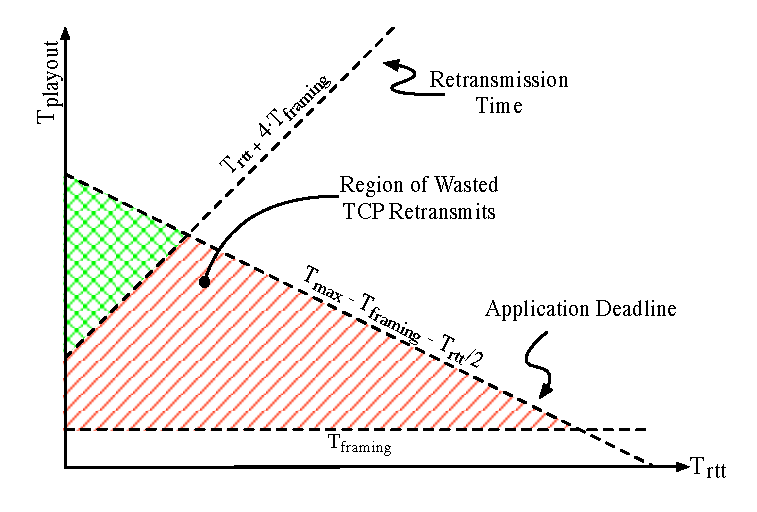
\includegraphics[width=\columnwidth]{figures/analysis-delay-region.pdf}
 \caption{\emph{Inconsistent Retransmissions} for real-time applications: TCP
 retransmissions may arrive too late to be used, if the play-out delay is set
  to meet the application deadline}
\label{diagram:inconsistentretrans}
\end{figure}

This inequality is shown graphically in Figure
\ref{diagram:inconsistentretrans}. The unshaded regions in Figure
\ref{diagram:inconsistentretrans} fall outside of the feasible operating regime
of the application and may be ignored, as they correspond to stalls in play-out
or overall delay bound violations.
% , and may be ignored: and are not part of the feasible operating regime of the
% application.
The feasible operating regime is represented by the shaded regions that separate
useful from wasteful retransmissions. The green cross-hatch highlights the
region where standard TCP retransmissions arrive in time to be useful.

Wasteful TCP retransmissions are marked by the red-lined region in
Figure~\ref{diagram:inconsistentretrans}. When the media play-out delay is less
than the retransmission time ($T_\mathrm{playout} < T_\mathrm{rexmit}$) but
satisfies the overall delay bound ($T_\mathrm{playout} \leq T_\mathrm{max} -
T_\mathrm{framing} - T_\mathrm{rtt}/2$),  and is greater than the framing
interval ($T_\mathrm{playout} \geq T_\mathrm{framing}$), then standard TCP
retransmissions will arrive too late.% to be useful.
% This region is marked with red stripes in
% Figure~\ref{diagram:inconsistentretrans}.
This is where inconsistent retransmissions are useful:
%However, this region can be used with inconsistent retransmissions:
when a TCP retransmission will arrive too late to replace the original lost
packet in this region. By contrast an inconsistent retransmission can use that
retransmission slot to transmit the next unsent data segment. The lost packet is
never recovered, but its sequence number is reused to send useful data.

\begin{table*}[h]
 \centering
 \normalsize
  \input{figures/analysis-utilitycompare.tex}
 \vspace{4mm}
 \caption{Sample TCP and TCP Hollywood RTT bounds required to meet application bounds,
 highlighting indicates where TCP Hollywood is beneficial}
\label{tab:analysis_comparison}
\end{table*}

\subsection{Inconsistent Retransmissions and Real-Time Media}
\label{subsec:realtime}
The benefits of TCP Hollywood can be quantified by substituting real-time
traffic parameters into Equation~\ref{eq:standard-rexmit}.
Consider interactive voice telephony. Widely deployed speech codecs typically
use $T_\mathrm{framing} = 20\mathrm{ms}$ with a delay bound of $T_\mathrm{max} =
150\mathrm{ms}$~\cite{itu:2003:delay}. Assuming media encoding delays are
negligible, so that $T_\mathrm{sender} = T_\mathrm{framing}$, then the feasible
region where standard TCP retransmissions arrive in time to be useful can be
derived from Equation \ref{eq:standard-rexmit} as:
\begin{equation}
  130\mathrm{ms} - T_\mathrm{rtt}/2
  \geq
  T_\mathrm{playout}
  \geq
  T_\mathrm{rtt} + 80\mathrm{ms}
  \label{eq:telephony-delay-bound}
\end{equation}
which has valid solutions for $T_\mathrm{playout}$ provided $T_\mathrm{rtt} \leq
33.33\mathrm{ms}$. This round-trip time bound is low for wide-area networks. For
example, TCP retransmission would be useful for calls from the authors' homes
within Europe, but discarded during inter-continental calls.
%% MF- Eq3 cannot be used to solve inconsistent rexmits where T_playout
%%     must be less than rexmit AND less than deadline but \geq framing.
Figure~\ref{diagram:inconsistentretrans} shows TCP Hollywood
provides valid solutions for $T_\mathrm{playout}$ when $T_\mathrm{rtt} \leq
220\mathrm{ms}$, showing the utility of inconsistent retransmissions for this
application.

For on-demand streaming using MPEG DASH, the framing interval
and delay bounds are typically much larger.  A typical deployment today
might use an encoding segment size of $T_\mathrm{framing} = 2\mathrm{s}$,
and an overall delay bound of $T_\mathrm{max} = 30\mathrm{s}$. Assuming
$T_\mathrm{sender} = T_\mathrm{framing}$, and substituting into Equation
\ref{eq:standard-rexmit}, this permits valid solutions for
$T_\mathrm{playout}$ provided $T_\mathrm{rtt} \leq 13.33\mathrm{s}$,
giving no benefit from inconsistent retransmission.

These two applications represent extremes in
terms of latency bounds: voice telephony has tight latency bounds, while
those of on-demand video streaming are relaxed. We analyse a third
application: IPTV delivery using DASH. IPTV applications seek to minimise
\textit{zap time} (i.e., the total time taken between a viewer selecting
a channel, and content from that channel being displayed). Bouzakaria
et al. \cite{bouzakaria:2014:overhead} show that end-to-end latencies --
the time between encoding and decoding of a frame -- of less than 240ms
can be achieved using DASH. Using their techniques, segments are fragmented
into $200\mathrm{ms}$ chunks for delivery, giving
$T_\mathrm{sender} = T_\mathrm{framing} = 200\mathrm{ms}$. An overall delay
bound of $T_\mathrm{max} = 1\mathrm{s}$ allows for channel surfing to be
supported. Substituting these values into Equation \ref{eq:standard-rexmit},
we see that regular TCP retransmissions do not benefit this application for
any RTT values. In contrast, inconsistent retransmissions in TCP Hollywood can
be used when $T_\mathrm{rtt} \leq 1\mathrm{s}$.

Table \ref{tab:analysis_comparison} summarises the three applications considered.
Utility of inconsistent retransmission is seen to depend on
the latency bounds of the application. Interactive applications, where
the overall latency requirements are tight, can strongly benefit from
the ability to send new data in place of a retransmission, but those
applications with relaxed latency bounds find less benefit.
%-------------------------------------------------------------------------------

\begin{figure*}
\centering
  \subfloat[$T_\mathrm{playout}$ region where blocked segments will be
           delivered too late.]{
           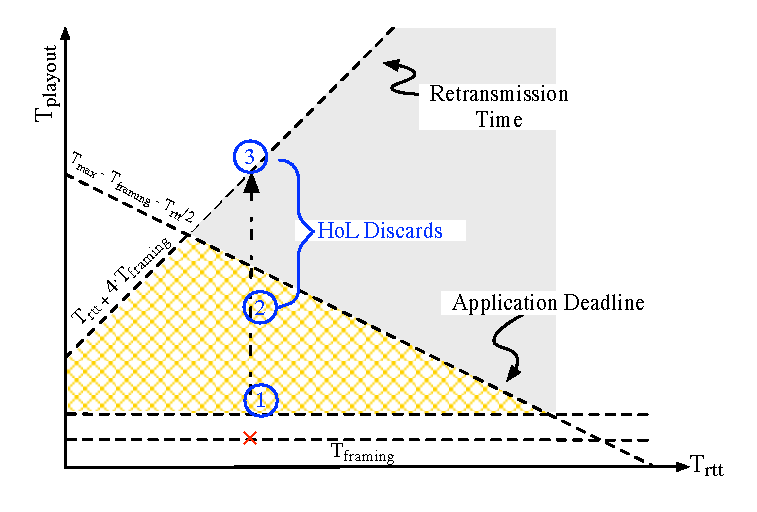
\includegraphics[width=\columnwidth]
           {figures/analysis-HoL-region-v2.pdf}
           \label{subfig:HoLregion}
  } \hfill
  \subfloat[Head of line blocking events between a loss and its
           retransmission.]{
           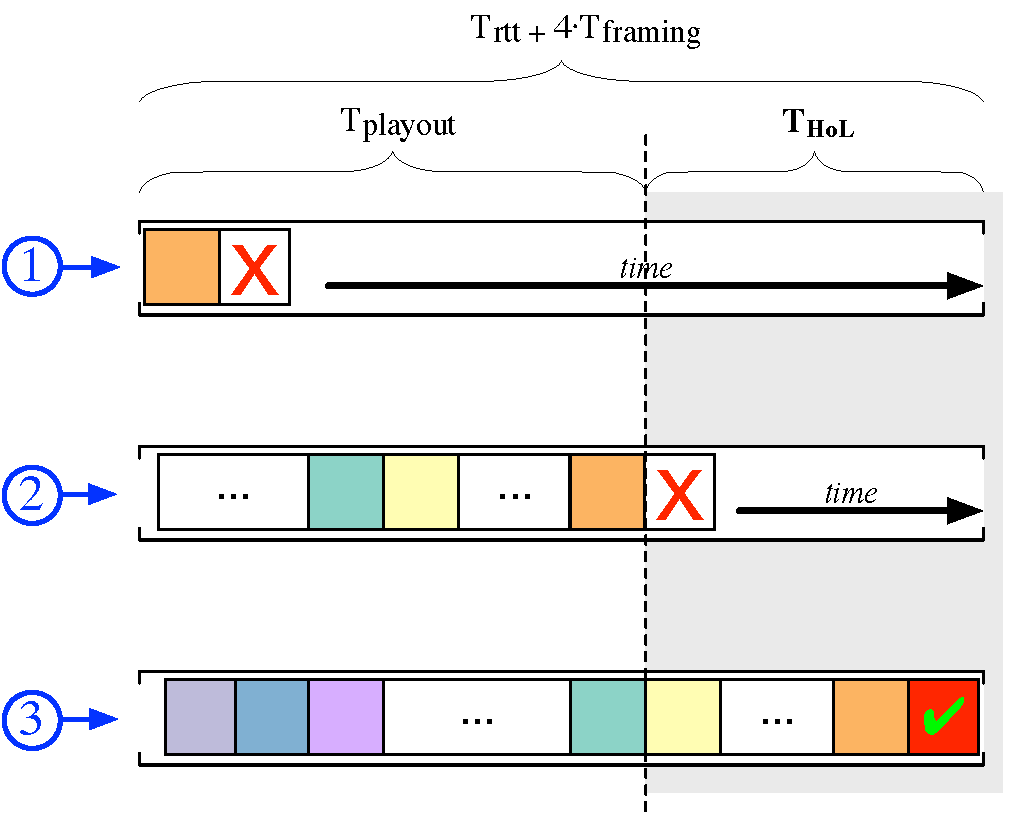
\includegraphics[width=0.9\columnwidth]
           {figures/analysis-HoL-time.pdf}
           \label{subfig:HoLtimed}
  }
 \caption{\emph{Head of line blocking} for real-time applications using regular TCP: for any given
 RTT and playout, segments that immediately follow a loss (1) are pushed
 past the acceptable deadline (2), and delivered as late as (3). The gap between RTT
 and playout is the duration of useful, but HoL blocked segments}
\label{fig:HoLanal}
\end{figure*}


%-------------------------------------------------------------------------------
\subsection{Connecting Head-of-Line Blocking}
\label{subsec:HoL}

If a packet is lost, then TCP will send a retransmission once a triple
duplicate ACK is received. If standard TCP is used, then later segments
will not be delivered to the application until the retransmission of the
lost segment is received, potentially causing media play-out to stall.
This is known as head-of-line blocking, as discussed in Section~\ref{sec:background}.

The size of the play-out buffer relative to the round-trip time and media
framing interval determines whether play-out stalls, or whether there is
sufficient buffering to cover the retransmission delay. From
Equation \ref{eq:playout_lower}, if
$T_\mathrm{playout} \geq T_\mathrm{rexmit} + T_\mathrm{framing}$, then the
retransmission will arrive in time to be played out, and no head-of-line
blocking will occur.

% Otherwise, there will be a period of duration $T_\mathrm{HoL} =
% T_\mathrm{rexmit} + T_\mathrm{framing} - T_\mathrm{playout}$ where the receiver
% is blocked waiting for the retransmission to arrive, and unable to play back
% media.
% %
% Substituting from Equation \ref{eq:retransmission}, this gives
% $T_\mathrm{HoL} = T_\mathrm{rtt} + 4 \times T_\mathrm{framing} -
% T_\mathrm{playout}$. If Equation \ref{eq:standard-rexmit} is satisfied,
% $T_\mathrm{HoL}$ is never positive, and the system cannot suffer from
% head-of-line blocking. If $T_\mathrm{playout}$ is below the minimum bound from
% Equation \ref{eq:standard-rexmit}, then head-of-line blocking can occur.
%
% =============

% TCP implements head-of-line blocking to facilitate in-order delivery. In the
% context of real-time traffic head-of-line blocking imposes additional delay on
% segments that follow a loss.
% Following from the previous discussion, a wasteful segment retransmission in TCP may
% cause some portion of blocked data, that otherwise arrives in time, to also
% become wasteful while waiting for the retransmission. Assuming no losses between
% a loss and its retransmission, then a full $T_\mathrm{rtt}$ of data will be
% delayed by head-of-line blocking. If $T_\mathrm{playout}$ adheres to the lower
% bound \todo{from equation ??} then all delayed segments will be delivered
% on time, despite the head-of-line blocking.

However, if $T_\mathrm{playout} < T_\mathrm{rexmit} + T_\mathrm{framing}$, then
the retransmission will not arrive in time to be played-out. This will cause a
1-segment gap in the media play-out, since some data is missing (this occurs
with both standard TCP, and with the TCP Hollywood extensions). If standard TCP
is used, then the receiver may \emph{also} suffer head-of-line blocking and be
unable to access later segments, leading to a longer gap in play-out.

If the retransmission arrives less than one framing interval after it was
scheduled to be played out, i.e., if
       $T_\mathrm{rexmit} \leq T_\mathrm{playout}
                          < T_\mathrm{rexmit} + T_\mathrm{framing}$
then it will arrive before the following packet is to be played.  In this case,
there is no head-of-line blocking, and only a single packet gap occurs in
play-out. If it is further delayed, such that $T_\mathrm{playout} <
T_\mathrm{rexmit}$, then head-of-line blocking will cause one or more later
frames to also miss their play-out.

A graphical representation is provided by Figure~\ref{fig:HoLanal}. The  yellow
cross-hatch region in Figure~\ref{subfig:HoLregion} is the region of
$T_\mathrm{playout}$ values where blocked segments will be made wasteful. The
details are labeled in Figure~\ref{subfig:HoLregion} by numbered events, with
associated time-lines in Figure~\ref{subfig:HoLtimed}. For a given value of
$T_\mathrm{rtt}$ the process begins with a loss marked by the red
`\textcolor{red}{$\times$}'. The next frame arrives at \textcircled{1} and is held by TCP,
as are all the segments that follow, awaiting the retransmission. For any size
of $T_\mathrm{playout}$ at that moment \textcircled{2}, the retransmission will arrive too
late. Upon arrival of the retransmission \textcircled{3} TCP releases blocked segments to
the play-out buffer. The duration of the head-of-line blocking that will be
discarded by the play-out buffer is labelled as $T_\mathrm{HoL}$ in
Figure~\ref{fig:HoLanal}, can be calculated as:
\begin{equation}
  T_\mathrm{HoL} = T_\mathrm{rexmit} - T_\mathrm{playout}
                 = T_\mathrm{rtt} + 3 \times T_\mathrm{framing} -
                 T_\mathrm{playout}
\label{eq:t-hol}
\end{equation}

The duration translates to $N_\mathrm{HoL}$ frames missing their play-out due to
head of line blocking, and in addition to the retransmission that arrived too
late, where:
\begin{equation}
  N_\mathrm{HoL} =
    \max\left(
      \left\lceil
      \frac{T_\mathrm{rtt} + 3 \times T_\mathrm{framing} - T_\mathrm{playout}}{T_\mathrm{framing}}
      \right\rceil, 0
    \right)
\label{eq:n-hol}
\end{equation}

% A graphical representation is provided by Figure~\ref{fig:HoLanal}.
% The  yellow cross-hatch region in Figure~\ref{subfig:HoLregion} is the region of
% $T_\mathrm{playout}$ values where blocked segments will be made wasteful.
%
% The details are labeled in Figure~\ref{subfig:HoLregion} by numbered events,
% with associated  time-lines in Figure~\ref{subfig:HoLtimed}. For a given value
% of $T_\mathrm{rtt}$ the process begins with a loss marked by the red
% '\textcolor{red}{$\times$}'. The next segment to arrive (1) is held by TCP, as
% are all segments that follow. Then for a given value of $T_\mathrm{playout}$ the
% retransmission (2) will arrive too late. TCP releases blocked segments upon (3)
% the arrival of the retransmission. The duration of blocked segments that will be
% discarded by the play-out buffer, labeled as $T_\mathrm{HoL}$ in
% Figure~\ref{fig:HoLanal}, can be calculated as
%
% \begin{align}
%   T_\mathrm{HoL} & = T_\mathrm{rexmit} - T_\mathrm{playout}
%                      \nonumber \\
%                  & = T_\mathrm{rtt} + 3 \times T_\mathrm{framing} - T_\mathrm{playout} .
% \label{eq:hol}
% \end{align}

Finally, we remark on the grey shaded region in Figure~\ref{subfig:HoLregion}
that occurs  when that when retransmissions arrive past the acceptable deadline.
From Equation~\ref{eq:standard-rexmit}, values of $T_\mathrm{playout}$ are
upper-bound by the application deadline. Subsituting this into
Equation~\ref{eq:t-hol} gives a lower bound on $T_\mathrm{HoL}$ of:
\begin{equation}
  T_\mathrm{HoL} \geq 3 \times T_\mathrm{rtt}/2 + 4 \times T_\mathrm{framing} - T_\mathrm{max}
\label{eq:hol-lower}
\end{equation}
%\begin{align}
%  T_\mathrm{HoL} & \geq T_\mathrm{rtt} + 4 \times T_\mathrm{framing}
%                        - T_\mathrm{max} - T_\mathrm{framing}
%                        - T_\mathrm{rtt}/2 \nonumber \\
%                 & \geq T_\mathrm{rtt}/2 + 3 \times T_\mathrm{framing}
%                        - T_\mathrm{max} .
%\label{eq:hol-lower}
%\end{align}
As $T_\mathrm{rtt}$ increases under TCP, so too does $T_\mathrm{HoL}$, and with
it the fragility of the real-time connection. While a TCP retransmission under
these circumstances will always arrive too late, the TCP Hollywood extensions eliminate
$T_\mathrm{HoL}$. In doing so the grey shaded region in
Figure~\ref{subfig:HoLregion}, where real-time connections may be infeasible
under TCP, are made viable with TCP Hollywood.

Our analysis identifies the value of inconsistent retransmissions, and the
way in which they interact with head-of-line blocking. Specifically, it
shows that removal of head-of-line blocking, via receiver side
modifications to the kernel TCP stack, is necessary to make effective use
of inconsistent retransmissions.  For this reason, a full deployment of
TCP Hollywood eliminates head-of-line blocking, to support latency
reduction and improve good-put due to inconsistent retransmissions.


%==================================================================================================
\section{Performance Evaluation}
\label{sec:perfeval}

% !TEX root = ../utltcp-paper.tex

In this section, we present initial performance evaluations. The primary goal 
is to show that the analysis presented in Section \ref{sec:analysis} holds,
while also showing that TCP Hollywood is useful for typical applications in realistic
network conditions.
We do this using the Mininet network emulator with a Linux implementation of TCP
Hollywood, simulating scenarios that represent typical networked multimedia
traffic from fixed-line residential networks.
This not only allows us to validate our analysis, but also can also form the
basis of future evaluation and deployment in the public Internet.


Section \ref{sec:simulator} describes the setup of the simulator used in the performance
evaluations, while Section \ref{sec:eval} discusses the parameters of the simulations,
and presents their results.

%--------------------------------------------------------------------------------------------------
\subsection{Simulator Setup}
\label{sec:simulator}

We use Mininet configured to emulate a dumbbell topology with a single bottleneck.
The bottleneck link of the dumbbell is an ADSL connection, with a download speed
of 8Mbps, and an upload speed of 1Mbps. ADSL is simulated because its use remains
widespread in large parts of the world, and is an environment where TCP Hollywood
is likely to show some benefit. The round-trip time is varied to allow exploration
of different behaviours, as will be discussed in Section \ref{sec:eval}.

We run TCP Hollywood flows representing the application under test, sharing the
bottleneck with cross-traffic. Three types of cross traffic are used:
single \emph{long-lived TCP} flows representing bulk downloads,
a bursty mix of short-lived TCP flows representing \emph{HTTP} traffic,
and multiple TCP connection representing an adaptive video download using
\emph{MPEG DASH}. Cross-traffic is used instead of a fixed random packet loss
rate; simulating such a loss rate is difficult, given the variability of
loss rates in the public Internet. Using different classes of typical cross
traffic is preferred.  We use the same parameters for generating cross
traffic for both protocols, but the simulations are non-deterministic so
the exact traffic pattern varies.

The Appendix further describes our choice of simulation parameters, the
rationale for our choice of simulation environment, and our approach to
ensuring reproducibility of results.

%--------------------------------------------------------------------------------------------------
\subsection{Evaluations}
\label{sec:eval}

In Section \ref{sec:analysis}, we showed how TCP and TCP Hollywood behaviour
splits into three regions, based on combinations of round-trip times and
play-out delays. In Figure \ref{diagram:inconsistentretrans}, these are
the green shaded
region, where TCP retransmissions are useful; the red shaded region, where TCP
retransmissions are not useful, but inconsistent retransmissions may be
beneficial; and finally, the unshaded region where no useful data can be
delivered -- the application is operating outside of its latency bounds.

\begin{figure}[t!]
	\includegraphics[width=\columnwidth]{figures/analysis-voip-inconsistent_region.pdf}
    \caption{Scenarios selected for VoIP application performance evaluations}
   	\label{fig:analysis-voip}
\end{figure}

Figure \ref{fig:analysis-voip} plots the same diagram, parameterised for the
Voice-over-IP application described in Section \ref{sec:analysis}, where
160-byte messages are sent every 20ms, to simulate the G.711 codec.
To validate the analysis, we simulate three scenarios using a round-trip time of
20ms and varying play-out delays:
(I) with play-out delay of
150ms, out-with the maximum delay tolerated by the application. At (II), the play-out delay
is 110ms; regular TCP and TCP Hollywood should provide the same timely goodput. At (III),
the play-out delay is 60ms, where TCP Hollywood should provide an increase in timely
goodput vs. standard TCP.
For each network scenario, and cross-traffic class, we plot:
\begin{itemize}
\item \emph{Timely good-put}:
                    TCP Hollywood is designed to improve performance by (i)
                    removing head-of-line blocking to reduce
                    latency; and (ii) introducing partial reliability to
                    increase utility.  Application-layer
                    latency (i.e., the time between the application sending
                    and receiving a message) gives insight into the
                    performance benefits, but fails to assess the trade-off
                    that TCP Hollywood makes between reliability and
                    timeliness.  Accordingly, we measure \emph{timely
                    good-put}, the rate at which useful bytes arrive at
                    the receiver. We define useful bytes as those that
                    arrive in time to be played out by the multimedia
                    application, with the correct timing to match the rest
                    of the media stream, and that have not already been
                    received.
\item \emph{Playout}: State of message playout for standard TCP and TCP Hollywood.
                    Messages that are successfully played out are shown in green; messages
                    that have expired (i.e., exceeded their maximum time bound) before their
                    play-out are shown in purple, and messages that arrived after their
                    play-out time are shown in orange. This plot begins when play-out starts,
                    removing the impact of the play-out buffer.
\item \emph{Latency}: Per-message latency for standard TCP and TCP Hollywood.
                    The latency of each message as it arrives at the application-layer is
                    shown. The sending application sends the message with a timestamp,
                    and the latency is determined at the receiver by comparing this to the
                    current time. Since simulations are performed on a
                    single host with Mininet, clocks are synchronised.
\item \emph{Segments}: Segment arrival for standard TCP and TCP Hollywood.
                    Segments that arrive in order are plotted in green. Segments that
                    arrive out-of-order are plotted in orange. Segments that fill an
                    earlier gap (i.e., retransmissions) are shown in purple. Segments that
                    were sent as inconsistent retransmissions are shown in blue, and are
                    additionally highlighted with marks on the border of the plot.
\end{itemize}

\begin{figure*}[t!]
\captionsetup[subfigure]{labelformat=empty}
\subfloat[Long-lived TCP]{\parbox{66mm}{
\begin{minipage}{5mm}
\rotatebox{90}{Timely goodput}
\end{minipage}
\begin{minipage}{61mm}
\includegraphics[width=61mm]{figures/perf-voip-adsl-uk-pd150ms-i-tg.pdf}\vspace{1mm}
\end{minipage}
\begin{minipage}{61mm}~\end{minipage}
}}
\subfloat[HTTP]{\parbox{61mm}{
\begin{minipage}{61mm}
\includegraphics[width=61mm]{figures/perf-voip-adsl-uk-pd150ms-ii-tg.pdf}\vspace{1mm}
\end{minipage}
\begin{minipage}{61mm}~\end{minipage}
}}
\subfloat[MPEG-DASH]{\parbox{61mm}{
\begin{minipage}{61mm}
\includegraphics[width=61mm]{figures/perf-voip-adsl-uk-pd150ms-iii-tg.pdf}\vspace{1mm}
\end{minipage}
\begin{minipage}{61mm}~\end{minipage}
}}
\caption{VoIP Scenario I: Timely goodput for standard TCP (Figure \ref{fig:voip-150-tcp}) and
                          TCP Hollywood (Figure \ref{fig:voip-150-tcph})}
\label{fig:voip-150-tg}
\end{figure*}

\begin{figure*}[t!]
\captionsetup[subfigure]{labelformat=empty}
\subfloat[Long-lived TCP]{\parbox{66mm}{
\begin{minipage}{5mm}
\rotatebox{90}{Playout}
\end{minipage}
\begin{minipage}{61mm}
\includegraphics[width=61mm]{figures/perf-voip-adsl-uk-pd150ms-i-tcp-playout.pdf}\vspace{1mm}
\end{minipage}
\begin{minipage}{5mm}
\rotatebox{90}{Message latency}
\end{minipage}
\begin{minipage}{61mm}
\includegraphics[width=61mm]{figures/perf-voip-adsl-uk-pd150ms-i-tcp-latency.pdf}\vspace{1mm}
\end{minipage}
\begin{minipage}{5mm}
\rotatebox{90}{Segments}
\end{minipage}
\begin{minipage}{61mm}
\includegraphics[width=61mm]{figures/perf-voip-adsl-uk-pd150ms-i-tcp-barcode.pdf}\vspace{1mm}
\end{minipage}
\begin{minipage}{61mm}~\end{minipage}
}}
\subfloat[HTTP]{\parbox{61mm}{
\begin{minipage}{61mm}
\includegraphics[width=61mm]{figures/perf-voip-adsl-uk-pd150ms-ii-tcp-playout.pdf}\vspace{1mm}
\end{minipage}
\begin{minipage}{61mm}
\includegraphics[width=61mm]{figures/perf-voip-adsl-uk-pd150ms-ii-tcp-latency.pdf}\vspace{1mm}
\end{minipage}
\begin{minipage}{61mm}
\includegraphics[width=61mm]{figures/perf-voip-adsl-uk-pd150ms-ii-tcp-barcode.pdf}\vspace{1mm}
\end{minipage}
\begin{minipage}{61mm}~\end{minipage}
}}
\subfloat[MPEG-DASH]{\parbox{61mm}{
\begin{minipage}{61mm}
\includegraphics[width=61mm]{figures/perf-voip-adsl-uk-pd150ms-iii-tcp-playout.pdf}\vspace{1mm}
\end{minipage}
\begin{minipage}{61mm}
\includegraphics[width=61mm]{figures/perf-voip-adsl-uk-pd150ms-iii-tcp-latency.pdf}\vspace{1mm}
\end{minipage}
\begin{minipage}{61mm}
\includegraphics[width=61mm]{figures/perf-voip-adsl-uk-pd150ms-iii-tcp-barcode.pdf}\vspace{1mm}
\end{minipage}
\begin{minipage}{61mm}~\end{minipage}
}}
\caption{VoIP Scenario I: Play-out buffer, message latencies, and segment arrival plots for standard TCP}
\label{fig:voip-150-tcp}
\end{figure*}

\begin{figure*}[t!]
\captionsetup[subfigure]{labelformat=empty}
\subfloat[Long-lived TCP]{\parbox{66mm}{
\begin{minipage}{5mm}
\rotatebox{90}{Playout}
\end{minipage}
\begin{minipage}{61mm}
\includegraphics[width=61mm]{figures/perf-voip-adsl-uk-pd150ms-i-tcph-playout.pdf}\vspace{1mm}
\end{minipage}
\begin{minipage}{5mm}
\rotatebox{90}{Message latency}
\end{minipage}
\begin{minipage}{61mm}
\includegraphics[width=61mm]{figures/perf-voip-adsl-uk-pd150ms-i-tcph-latency.pdf}\vspace{1mm}
\end{minipage}
\begin{minipage}{5mm}
\rotatebox{90}{Segments}
\end{minipage}
\begin{minipage}{61mm}
\includegraphics[width=61mm]{figures/perf-voip-adsl-uk-pd150ms-i-tcph-barcode.pdf}\vspace{1mm}
\end{minipage}
\begin{minipage}{61mm}~\end{minipage}
}}
\subfloat[HTTP]{\parbox{61mm}{
\begin{minipage}{61mm}
\includegraphics[width=61mm]{figures/perf-voip-adsl-uk-pd150ms-ii-tcph-playout.pdf}\vspace{1mm}
\end{minipage}
\begin{minipage}{61mm}
\includegraphics[width=61mm]{figures/perf-voip-adsl-uk-pd150ms-ii-tcph-latency.pdf}\vspace{1mm}
\end{minipage}
\begin{minipage}{61mm}
\includegraphics[width=61mm]{figures/perf-voip-adsl-uk-pd150ms-ii-tcph-barcode.pdf}\vspace{1mm}
\end{minipage}
\begin{minipage}{61mm}~\end{minipage}
}}
\subfloat[MPEG-DASH]{\parbox{61mm}{
\begin{minipage}{61mm}
\includegraphics[width=61mm]{figures/perf-voip-adsl-uk-pd150ms-iii-tcph-playout.pdf}\vspace{1mm}
\end{minipage}
\begin{minipage}{61mm}
\includegraphics[width=61mm]{figures/perf-voip-adsl-uk-pd150ms-iii-tcph-latency.pdf}\vspace{1mm}
\end{minipage}
\begin{minipage}{61mm}
\includegraphics[width=61mm]{figures/perf-voip-adsl-uk-pd150ms-iii-tcph-barcode.pdf}\vspace{1mm}
\end{minipage}
\begin{minipage}{61mm}~\end{minipage}
}}
\caption{VoIP Scenario I: Play-out buffer, message latencies, and segment arrival plots for TCP Hollywood}
\label{fig:voip-150-tcph}
\end{figure*}

The simulation results for Scenario I are shown in Figures \ref{fig:voip-150-tg},
\ref{fig:voip-150-tcp}, and \ref{fig:voip-150-tcph}.
There are three groups of results:
Figure \ref{fig:voip-150-tg} shows timely goodput for both standard TCP and
for TCP Hollywood competing with each of the three types of cross traffic.
Figure \ref{fig:voip-150-tcp} shows, for standard TCP, and with each type
of cross traffic, whether segments were played out on time (top), the per
message latency as measured at the application layer (middle), and whether
each segment was received, retransmitted, or inconsistently retransmitted
(bottomw).
Finally, Figure \ref{fig:voip-150-tcph}, plots the same information, but
for TCP Hollywood.

\begin{figure*}[t!]
\captionsetup[subfigure]{labelformat=empty}
\subfloat[Long-lived TCP]{\parbox{66mm}{
\begin{minipage}{5mm}
\rotatebox{90}{Timely goodput}
\end{minipage}
\begin{minipage}{61mm}
\includegraphics[width=61mm]{figures/perf-voip-adsl-uk-pd110ms-i-tg.pdf}\vspace{1mm}
\end{minipage}
\begin{minipage}{61mm}~\end{minipage}
}}
\subfloat[HTTP]{\parbox{61mm}{
\begin{minipage}{61mm}
\includegraphics[width=61mm]{figures/perf-voip-adsl-uk-pd110ms-ii-tg.pdf}\vspace{1mm}
\end{minipage}
\begin{minipage}{61mm}~\end{minipage}
}}
\subfloat[MPEG-DASH]{\parbox{61mm}{
\begin{minipage}{61mm}
\includegraphics[width=61mm]{figures/perf-voip-adsl-uk-pd110ms-iii-tg.pdf}\vspace{1mm}
\end{minipage}
\begin{minipage}{61mm}~\end{minipage}
}}
\caption{VoIP Scenario II: Timely goodput for standard TCP (Figure \ref{fig:voip-110-tcp}) and
                          TCP Hollywood (Figure \ref{fig:voip-110-tcph})}
\label{fig:voip-110-tg}
\end{figure*}

\begin{figure*}[t!]
\captionsetup[subfigure]{labelformat=empty}
\subfloat[Long-lived TCP]{\parbox{66mm}{
\begin{minipage}{5mm}
\rotatebox{90}{Playout}
\end{minipage}
\begin{minipage}{61mm}
\includegraphics[width=61mm]{figures/perf-voip-adsl-uk-pd110ms-i-tcp-playout.pdf}\vspace{1mm}
\end{minipage}
\begin{minipage}{5mm}
\rotatebox{90}{Message latency}
\end{minipage}
\begin{minipage}{61mm}
\includegraphics[width=61mm]{figures/perf-voip-adsl-uk-pd110ms-i-tcp-latency.pdf}\vspace{1mm}
\end{minipage}
\begin{minipage}{5mm}
\rotatebox{90}{Segments}
\end{minipage}
\begin{minipage}{61mm}
\includegraphics[width=61mm]{figures/perf-voip-adsl-uk-pd110ms-i-tcp-barcode.pdf}\vspace{1mm}
\end{minipage}
\begin{minipage}{61mm}~\end{minipage}
}}
\subfloat[HTTP]{\parbox{61mm}{
\begin{minipage}{61mm}
\includegraphics[width=61mm]{figures/perf-voip-adsl-uk-pd110ms-ii-tcp-playout.pdf}\vspace{1mm}
\end{minipage}
\begin{minipage}{61mm}
\includegraphics[width=61mm]{figures/perf-voip-adsl-uk-pd110ms-ii-tcp-latency.pdf}\vspace{1mm}
\end{minipage}
\begin{minipage}{61mm}
\includegraphics[width=61mm]{figures/perf-voip-adsl-uk-pd110ms-ii-tcp-barcode.pdf}\vspace{1mm}
\end{minipage}
\begin{minipage}{61mm}~\end{minipage}
}}
\subfloat[MPEG-DASH]{\parbox{61mm}{
\begin{minipage}{61mm}
\includegraphics[width=61mm]{figures/perf-voip-adsl-uk-pd110ms-iii-tcp-playout.pdf}\vspace{1mm}
\end{minipage}
\begin{minipage}{61mm}
\includegraphics[width=61mm]{figures/perf-voip-adsl-uk-pd110ms-iii-tcp-latency.pdf}\vspace{1mm}
\end{minipage}
\begin{minipage}{61mm}
\includegraphics[width=61mm]{figures/perf-voip-adsl-uk-pd110ms-iii-tcp-barcode.pdf}\vspace{1mm}
\end{minipage}
\begin{minipage}{61mm}~\end{minipage}
}}
\caption{VoIP Scenario II: Play-out buffer, message latencies, and segment arrival plots for standard TCP}
\label{fig:voip-110-tcp}
\end{figure*}

\begin{figure*}[t!]
\captionsetup[subfigure]{labelformat=empty}
\subfloat[Long-lived TCP]{\parbox{66mm}{
\begin{minipage}{5mm}
\rotatebox{90}{Playout}
\end{minipage}
\begin{minipage}{61mm}
\includegraphics[width=61mm]{figures/perf-voip-adsl-uk-pd110ms-i-tcph-playout.pdf}\vspace{1mm}
\end{minipage}
\begin{minipage}{5mm}
\rotatebox{90}{Message latency}
\end{minipage}
\begin{minipage}{61mm}
\includegraphics[width=61mm]{figures/perf-voip-adsl-uk-pd110ms-i-tcph-latency.pdf}\vspace{1mm}
\end{minipage}
\begin{minipage}{5mm}
\rotatebox{90}{Segments}
\end{minipage}
\begin{minipage}{61mm}
\includegraphics[width=61mm]{figures/perf-voip-adsl-uk-pd110ms-i-tcph-barcode.pdf}\vspace{1mm}
\end{minipage}
\begin{minipage}{61mm}~\end{minipage}
}}
\subfloat[HTTP]{\parbox{61mm}{
\begin{minipage}{61mm}
\includegraphics[width=61mm]{figures/perf-voip-adsl-uk-pd110ms-ii-tcph-playout.pdf}\vspace{1mm}
\end{minipage}
\begin{minipage}{61mm}
\includegraphics[width=61mm]{figures/perf-voip-adsl-uk-pd110ms-ii-tcph-latency.pdf}\vspace{1mm}
\end{minipage}
\begin{minipage}{61mm}
\includegraphics[width=61mm]{figures/perf-voip-adsl-uk-pd110ms-ii-tcph-barcode.pdf}\vspace{1mm}
\end{minipage}
\begin{minipage}{61mm}~\end{minipage}
}}
\subfloat[MPEG-DASH]{\parbox{61mm}{
\begin{minipage}{61mm}
\includegraphics[width=61mm]{figures/perf-voip-adsl-uk-pd110ms-iii-tcph-playout.pdf}\vspace{1mm}
\end{minipage}
\begin{minipage}{61mm}
\includegraphics[width=61mm]{figures/perf-voip-adsl-uk-pd110ms-iii-tcph-latency.pdf}\vspace{1mm}
\end{minipage}
\begin{minipage}{61mm}
\includegraphics[width=61mm]{figures/perf-voip-adsl-uk-pd110ms-iii-tcph-barcode.pdf}\vspace{1mm}
\end{minipage}
\begin{minipage}{61mm}~\end{minipage}
}}
\caption{VoIP Scenario II: Play-out buffer, message latencies, and segment arrival plots for TCP Hollywood}
\label{fig:voip-110-tcph}
\end{figure*}


% ================


\begin{figure*}[t!]
\captionsetup[subfigure]{labelformat=empty}
\subfloat[Long-lived TCP]{\parbox{66mm}{
\begin{minipage}{5mm}
\rotatebox{90}{Timely goodput}
\end{minipage}
\begin{minipage}{61mm}
\includegraphics[width=61mm]{figures/perf-voip-adsl-uk-pd60ms-i-tg.pdf}\vspace{1mm}
\end{minipage}
\begin{minipage}{61mm}~\end{minipage}
}}
\subfloat[HTTP]{\parbox{61mm}{
\begin{minipage}{61mm}
\includegraphics[width=61mm]{figures/perf-voip-adsl-uk-pd60ms-ii-tg.pdf}\vspace{1mm}
\end{minipage}
\begin{minipage}{61mm}~\end{minipage}
}}
\subfloat[MPEG-DASH]{\parbox{61mm}{
\begin{minipage}{61mm}
\includegraphics[width=61mm]{figures/perf-voip-adsl-uk-pd60ms-iii-tg.pdf}\vspace{1mm}
\end{minipage}
\begin{minipage}{61mm}~\end{minipage}
}}
\caption{VoIP Scenario III: Timely goodput for standard TCP (Figure \ref{fig:voip-60-tcp}) and
                          TCP Hollywood (Figure \ref{fig:voip-60-tcph})}
\label{fig:voip-60-tg}
\end{figure*}

\begin{figure*}[t!]
\captionsetup[subfigure]{labelformat=empty}
\subfloat[Long-lived TCP]{\parbox{66mm}{
\begin{minipage}{5mm}
\rotatebox{90}{Playout}
\end{minipage}
\begin{minipage}{61mm}
\includegraphics[width=61mm]{figures/perf-voip-adsl-uk-pd60ms-i-tcp-playout.pdf}\vspace{1mm}
\end{minipage}
\begin{minipage}{5mm}
\rotatebox{90}{Message latency}
\end{minipage}
\begin{minipage}{61mm}
\includegraphics[width=61mm]{figures/perf-voip-adsl-uk-pd60ms-i-tcp-latency.pdf}\vspace{1mm}
\end{minipage}
\begin{minipage}{5mm}
\rotatebox{90}{Segments}
\end{minipage}
\begin{minipage}{61mm}
\includegraphics[width=61mm]{figures/perf-voip-adsl-uk-pd60ms-i-tcp-barcode.pdf}\vspace{1mm}
\end{minipage}
\begin{minipage}{61mm}~\end{minipage}
}}
\subfloat[HTTP]{\parbox{61mm}{
\begin{minipage}{61mm}
\includegraphics[width=61mm]{figures/perf-voip-adsl-uk-pd60ms-ii-tcp-playout.pdf}\vspace{1mm}
\end{minipage}
\begin{minipage}{61mm}
\includegraphics[width=61mm]{figures/perf-voip-adsl-uk-pd60ms-ii-tcp-latency.pdf}\vspace{1mm}
\end{minipage}
\begin{minipage}{61mm}
\includegraphics[width=61mm]{figures/perf-voip-adsl-uk-pd60ms-ii-tcp-barcode.pdf}\vspace{1mm}
\end{minipage}
\begin{minipage}{61mm}~\end{minipage}
}}
\subfloat[MPEG-DASH]{\parbox{61mm}{
\begin{minipage}{61mm}
\includegraphics[width=61mm]{figures/perf-voip-adsl-uk-pd60ms-iii-tcp-playout.pdf}\vspace{1mm}
\end{minipage}
\begin{minipage}{61mm}
\includegraphics[width=61mm]{figures/perf-voip-adsl-uk-pd60ms-iii-tcp-latency.pdf}\vspace{1mm}
\end{minipage}
\begin{minipage}{61mm}
\includegraphics[width=61mm]{figures/perf-voip-adsl-uk-pd60ms-iii-tcp-barcode.pdf}\vspace{1mm}
\end{minipage}
\begin{minipage}{61mm}~\end{minipage}
}}
\caption{VoIP Scenario III: Play-out buffer, message latencies, and segment arrival plots for standard TCP}
\label{fig:voip-60-tcp}
\end{figure*}

\begin{figure*}[t!]
\captionsetup[subfigure]{labelformat=empty}
\subfloat[Long-lived TCP]{\parbox{66mm}{
\begin{minipage}{5mm}
\rotatebox{90}{Playout}
\end{minipage}
\begin{minipage}{61mm}
\includegraphics[width=61mm]{figures/perf-voip-adsl-uk-pd60ms-i-tcph-playout.pdf}\vspace{1mm}
\end{minipage}
\begin{minipage}{5mm}
\rotatebox{90}{Message latency}
\end{minipage}
\begin{minipage}{61mm}
\includegraphics[width=61mm]{figures/perf-voip-adsl-uk-pd60ms-i-tcph-latency.pdf}\vspace{1mm}
\end{minipage}
\begin{minipage}{5mm}
\rotatebox{90}{Segments}
\end{minipage}
\begin{minipage}{61mm}
\includegraphics[width=61mm]{figures/perf-voip-adsl-uk-pd60ms-i-tcph-barcode.pdf}\vspace{1mm}
\end{minipage}
\begin{minipage}{61mm}~\end{minipage}
}}
\subfloat[HTTP]{\parbox{61mm}{
\begin{minipage}{61mm}
\includegraphics[width=61mm]{figures/perf-voip-adsl-uk-pd60ms-ii-tcph-playout.pdf}\vspace{1mm}
\end{minipage}
\begin{minipage}{61mm}
\includegraphics[width=61mm]{figures/perf-voip-adsl-uk-pd60ms-ii-tcph-latency.pdf}\vspace{1mm}
\end{minipage}
\begin{minipage}{61mm}
\includegraphics[width=61mm]{figures/perf-voip-adsl-uk-pd60ms-ii-tcph-barcode.pdf}\vspace{1mm}
\end{minipage}
\begin{minipage}{61mm}~\end{minipage}
}}
\subfloat[MPEG-DASH]{\parbox{61mm}{
\begin{minipage}{61mm}
\includegraphics[width=61mm]{figures/perf-voip-adsl-uk-pd60ms-iii-tcph-playout.pdf}\vspace{1mm}
\end{minipage}
\begin{minipage}{61mm}
\includegraphics[width=61mm]{figures/perf-voip-adsl-uk-pd60ms-iii-tcph-latency.pdf}\vspace{1mm}
\end{minipage}
\begin{minipage}{61mm}
\includegraphics[width=61mm]{figures/perf-voip-adsl-uk-pd60ms-iii-tcph-barcode.pdf}\vspace{1mm}
\end{minipage}
\begin{minipage}{61mm}~\end{minipage}
}}
\caption{VoIP Scenario III: Play-out buffer, message latencies, and segment arrival plots for TCP Hollywood}
\label{fig:voip-60-tcph}
\end{figure*}

In scenario I, the combination of a 150ms play-out delay and 10ms network
delay (20ms RTT) is chosen such that the application is operating beyond
its maximum one-way delay bound. That is, packets cannot arrive in time to
meet the deadline, irrespective of whether standard TCP or TCP Hollywood
are used. This is clear in the figures: the timely goodput (Figure
\ref{fig:voip-150-tg}) is zero for both protocols, and the playout plots
show all messages have expired.  Both standard TCP and TCP Hollywood behave
as expected: playout in this scenario is not feasible for either protocol.

The results for Scenario II are shown in Figures \ref{fig:voip-110-tg},
\ref{fig:voip-110-tcp}, and \ref{fig:voip-110-tcph}.
Figure \ref{fig:voip-110-tg} plots the timely goodput for both standard TCP
and TCP Hollywood, while Figures \ref{fig:voip-110-tcp} and \ref{fig:voip-110-tcph} 
show the playout of the segments, application-layer message latency, and
segment arrivals for the two protocols. Each figure shows performance with
each of the three types of cross traffic. 

In this scenario, the playout delay is set to 110ms, chosen such that the
combination of playout delay and network round-trip time allows
retransmissions to arrive before the lost and retransmitted segment is 
due to be played out. Accordingly, the performance of standard TCP and 
TCP Hollywood should be comparable. We see this in the figures. While
there is variation in the timely goodput (Figure \ref{fig:voip-110-tg}) 
due to variations in the cross traffic, there is no significant difference
between standard TCP and TCP Hollywood. The other metrics (Figures 
\ref{fig:voip-110-tcp} and \ref{fig:voip-110-tcph}) are also comparable,
although since the pattern of segment arrivals varies depending on the
cross traffic, we see differences in instantaneous message latency and
playout.


\begin{figure*}[t!]
\captionsetup[subfigure]{labelformat=empty}
\subfloat[\hspace{5mm}(i) Standard TCP]{\parbox{96mm}{
\begin{minipage}{5mm}
\rotatebox{90}{Playout}
\end{minipage}
\begin{minipage}{91mm}
\includegraphics[width=91mm]{figures/perf-playout-voip-tcp-zoom.pdf}\vspace{1mm}
\end{minipage}
\begin{minipage}{5mm}
\rotatebox{90}{Message latency}
\end{minipage}
\begin{minipage}{91mm}
\includegraphics[width=91mm]{figures/perf-latency-voip-tcp-zoom.pdf}\vspace{1mm}
\end{minipage}
\begin{minipage}{5mm}
\rotatebox{90}{Segments}
\end{minipage}
\begin{minipage}{91mm}
\includegraphics[width=91mm]{figures/perf-barcode-voip-tcp-zoom.pdf}\vspace{1mm}
\end{minipage}
\begin{minipage}{91mm}~\end{minipage}
}}
\subfloat[(ii) TCP Hollywood]{\parbox{91mm}{
\begin{minipage}{91mm}
\includegraphics[width=91mm]{figures/perf-playout-voip-tcph-zoom.pdf}\vspace{1mm}
\end{minipage}
\begin{minipage}{91mm}
\includegraphics[width=91mm]{figures/perf-latency-voip-tcph-zoom.pdf}\vspace{1mm}
\end{minipage}
\begin{minipage}{91mm}
\includegraphics[width=91mm]{figures/perf-barcode-voip-tcph-zoom.pdf}\vspace{1mm}
\end{minipage}
\begin{minipage}{91mm}~\end{minipage}
}}
\caption{VoIP: comparing the behaviour of standard TCP and TCP Hollywood when a segment is lost}
\label{fig:voip-comparison}
\end{figure*}

Figure \ref{fig:voip-110-tcph} also demonstrates a sensitivity of TCP
Hollywood to the accuracy of the TCP RTT estimate. The segment plots
show a significant number of inconsistent retransmissions, marked by
ticks on the outside of the plots. These are strongly correlated with
latency spikes, and occur when short-term increases in delay push the
delivery time estimate for the packets past their deadline, causing
TCP Hollywood to send inconsistent retransmissions.
We believe the spikes in latency due to queuing are causing the playout
time of the packets to oscillate around their deadline. Sometimes this
hurts TCP Hollywood, since inconsistent retransmissions are incorrectly
sent; equally, though, it hurts standard TCP since there are times where
inconsistent retransmissions are needed.  There is no significant impact 
on the timely goodput.

Finally, the results for Scenario III are shown in Figures
\ref{fig:voip-60-tg}, \ref{fig:voip-60-tcp}, and \ref{fig:voip-60-tcph}.
This is the primary scenario of interest: the combination of playout delay
and network round trip time is such that standard retransmissions will not
arrive in time to be played out, causing head-of-line blocking that will
affect performance with standard TCP. In contrast, the use of inconsistent
retransmissions and an alternate, message based, API that avoids head of
line blocking should allow TCP Hollywood to perform well.

Considering the timely goodput, Figure \ref{fig:voip-60-tg}, we see that
both protocols are comparable when network conditions
are good. However, with long-lived TCP cross traffic and MPEG DASH cross
traffic, there are several regions where the timely goodput of standard
TCP drops sharply below that of TCP Hollywood. It can readily be seen 
that these correlate with the spikes in Message Latency seen in Figure
\ref{fig:voip-60-tcp}. The corresponding spikes in latency for the TCP
Hollywood traces, Figure \ref{fig:voip-60-tcph}, do not show the drop
in timely goodput, but do correlate with inconsistent retransmissions.
This is the behaviour we expect: standard TCP flows stall due to head
of line blocking with waiting for retransmissions that arrive too late
to be played out, while TCP Hollywood sends an inconsistent retransmission
that arrives in time to be useful. The TCP Hollywood receiver sees a burst
of packet loss, while the standard TCP receiver sees no loss, but a longer
burst of packets being delivered late. TCP Hollywood achieves better
\emph{timely} goodput, even though the amount of packet loss at the
application is higher. 

The behaviour of standard TCP and TCP Hollywood in the case of segment loss
is explored in more detail in Figure \ref{fig:voip-comparison}.  The loss
events are drawn from the Scenario III long-lived TCP plots, at around 108
seconds for standard TCP and 84 seconds for TCP Hollywood.  
Impact of removing head-of-line blocking is clear: fewer of the messages
preceding the delivery of a retransmission miss their deadline.
% FIXME: this should be expanded

% \todo{Discuss inconsistent retransmissions once plotted}
% \todo{Has it been checked that these are actual inconsistent retransmissions yet?}
% 
% plot the timely goodput, and playout, latency, and barcode plots for TCP
% and TCP Hollywood for Scenario III. On average, TCP Hollywood achieves more
% timely goodput than standard TCP.  \todo{expand this}
% 
% \todo{Add numbers to support this.}
% 
% \begin{table*}[h]
%  \centering
%  \normalsize
%   \input{figures/perfeval-results.tex}
%  \vspace{4mm}
%   \caption{Performance evaluation results}
% \label{tab:perfeval-results}
% \end{table*}
% FIXME: This table is not especially meaningful, since it's missing
% confidence intervals. Need to re-run the simulations enough to get
% meaningful error bar statistics. 


In summary, this performance evaluation shows the validity of the
analysis presented in Section \ref{sec:analysis}. TCP Hollywood is shown
to improve timely goodput in cases where standard TCP retransmissions would
arrive too late to be useful, converting a long duration playout stall into 
a shorter packet loss event.



%==================================================================================================

\section{Feasibility of Deployment}
\label{sec:deployability}

% !TEX root = ../utltcp-paper.tex

% The design of TCP Hollywood makes only one wire-visible modification to TCP:
% inconsistent retransmissions. Middleboxes along the path may see multiple
%segments with the same TCP sequence number, but with different payloads.

% We investigate the feasibility of deploying TCP Hollywood, using results
% from initial experiments with a FreeBSD implementation on
% residential and mobile networks in the UK.
%
% \todo{Remove reference to FreeBSD? Confuses the point?}

In an ossified Internet, TCP Hollywood must survive middlebox behaviours if it
is to be deployable. In this section we present positive results from a
preliminary investigation of TCP Hollyood between a residential and multiple
mobile networks in the UK.

TCP Hollywood is designed to be entirely compatible with TCP. The only
on-the-wire visible difference between a TCP Hollywood flow and a standard TCP
flow appears within the payload data carried by inconsistent retransmissions.
Recall from Section~\ref{subsec:sender} that inconsistent retransmissions carry
new payload data inside of segments with previously transmitted sequence
numbers. This modification is invisible to receivers and middleboxes that only
process TCP/IP headers, but is visible to middleboxes that use deep packet
inspection if they compare the contents of a retransmitted packet with the
original data. Depending on the configuration such behaviour may disrupt the
connection. For example, a firewall may interpret inconsistent retransmissions
as belonging to a man-on-the-side attack, and reset the connection.

We conducted experiments with a live deployment of TCP Hollywood to obtain an
initial assessment on whether such middleboxes exist, and what impact they have.
A TCP Hollywood server was setup on a public IP address. The server was
configured to always send inconsistent retransmissions in lieu of the original
data, so that all retransmissions contained new data with the same sequence
numbers. Listen ports were set as 80, 4001, and 5001. Port 80 is used by web
traffic, and can be expected to be affected by middleboxes such as
``transparent'' caches and firewalls. We expect ports 4001 and 5001 to be less
likely to be subject to interference by middleboxes, since they are not used by
popular applications.

% Port 5001 is used for control, i.e. with no induced loss.

% Clients were deployed across a number of access networks, operated by different
% service providers. Each
Clients connected to the server, and received data. All
incoming segments to the client host were recorded by \texttt{tcpdump}, then
filtered by \texttt{iptables} to uniformly drop 5\% of segments before reaching
the TCP stack for traffic from ports 80 and 4001. Traffic from port 5001 was
unaffected.\footnote{Given that our goal is to test the ability to deploy TCP
Hollywood, rather than performance, we are only concerned with creating
sufficient loss to trigger inconsistent retransmissions. A high
\emph{un-correlated} drop rate enables TCP to survive where it would fail
against correlated drops. The ensuing reduction in throughput translates to
reduced loss due to congestion. Thus the client is more likely to see both the
original transmission and its retransmission.} Each loss induced at the client
triggered an inconsistent retransmission from the server.
%The random drop ensured that the client TCP stack experienced loss, and
%triggered the retransmission of the lost segment from the server.
Remaining segments were passed up the stack to the client application, as
normal. Data received by the client application was recorded, and compared
against \texttt{tcpdump} logs from the server to identify the dropped
segments, and to compare the payload data in the dropped segments with
that sent in the original packet and in the inconsistent retransmission.
This allows us to see what segments have been dropped, and to confirm that
both the original and retransmission cross the path between client and
server, and whether the inconsistent retransmission was delivered.

The evaluation was conducted using clients in 14 different locations in the UK,
connecting to a server located at the University of Glasgow. The clients
connected via eight different fixed-line residential ISPs (Andrews \& Arnold,
BT, Demon, EE, Eclipse, Sky, TalkTalk, and Virgin), and four mobile operators
(EE, O2, Three, and Vodafone).  All of the fixed-line residential ISPs
successfully delivered the inconsistent retransmissions. Among the four mobile
operators, only one delivered inconsistent retransmissions. The three remaining
mobile operators delivered the original segments instead, yet the server saw no
corresponding segment loss. This observed behaviour is consistent with a
transparent split-connection TCP performance enhancing proxy cache that
intercepts and responds to ACKs from the client on behalf of the server. This
caching behaviour was observed on ports 80 and 4001 for two of the three
providers, while the other provider appeared to operate a cache on port 80 only.

Crucially, TCP Hollywood {\em continued to operate irrespective of middlebox
presence} in the network. At no time did connections suffer a reset, nor did the
use of the TCP Hollywood extensions affect connectivity or performance.
Middlebox manipulations such as caching are designed to be transparent, leaving
the client to believe it is interacting with a standard TCP server. Recall from
Section~\ref{subsec:partialdep} that TCP Hollywood is designed for partial
deployment. This experiment provides evidence that TCP Hollywood continues to
deliver messages and eliminate head-of-line blocking, even when inconsistent
retransmissions are absent. In the worst-case, performance is the same as TCP
without our extensions.

The set of networks tested is by no means exhaustive. Further, and larger scale,
evaluation is needed to build evidence that inconsistent retransmissions are
deployable. Previous studies provide room for optimism, however. Honda et al.
\cite{honda:2011:extend-tcp} investigated deployment of TCP modifications with
regards to middlebox interaction, from 142 networks in 24 countries, in early
2011, including inconsistent retransmission measurements taken over a large
number of paths, with path diversity. Their observations mirror ours: the
majority of paths deliver inconsistent retransmissions as expected, while a
small number deliver the original instead. They also observed connection resets
on one path, representing less than 1\% of paths evaluated.

%Some discussion about (hypothetical, unseen)
%middleboxes that might break the protocol? And checksumming/DTLS as a solution}


%==================================================================================================
\section{Related Work}
\label{sec:related}

% !TEX root = ../utltcp-paper.tex

The immediate precursors of TCP Hollywood are the Minion protocol suite
\cite{nowlan:2012:minion} and TL-TCP \cite{mukherjee:2000:timelines}. The
Minion protocol suite includes uTCP, which proves a COBS-encoded user-space
datagram abstraction atop TCP, with prioritization and out-of-order
delivery. uTCP also provides an API that enables applications to replace
existing datagrams in the transmission buffer before they are sent.
Datagrams that have already been sent (i.e., those being retransmitted)
cannot be replaced. The authors acknowledge this as a conservative design
choice, made to ensure middlebox interaction.

Our wire compatibility experiments from Section \ref{sec:deployability},
and those of Honda et al. \cite{honda:2011:extend-tcp}, indicate that
inconsistent retransmissions are possible, but that the integrity of the
sequence space needs to be preserved. The need to consider middlebox
interaction with new or modified protocols is underscored by the design,
and success, of Multi-Path TCP \cite{raiciu:2012:hard}. The design of
TCP Hollywood builds on a number of protocols, and tweaks to TCP, that are
unlikely to be deployable.

TL-TCP marks the first appearance of time-lines and
inconsistent retransmissions~\cite{mukherjee:2000:timelines}. The underlying
mechanism works by injecting gaps into the sequence space. This modification is
observable by middleboxes, and so is unlikely to be deployable. TCP Hollywood
builds on TL-TCP, and related protocols, but does so while focussing on
deployability. As discussed in Section \ref{sec:design}, we minimise changes
to the wire protocol to maximise
compatibility with middleboxes.

Transport protocols that rely on application-layer metadata to
improve performance include Partially Error Controlled Connection
(PECC)~\cite{dempsey:1992:adaptive} and PRTP-ECN~\cite{grinnemo:2001:prtp}.
Other protocols such as SCTP \cite{rfc:4960} and DCCP \cite{rfc:4340} were
engineered to broaden the delivery models offered by the transport-layer.
Despite standardization and deployment in mainstream operating systems, their
use is hampered by a lack of middlebox support.
% The main difference between these protocols and TCP Hollywood is the focus on
% deployability: middlebox interaction must be considered.

Liang and Cheriton in~\cite{liang:2002:tcp-rtm} note that loss can be more detrimental
to streaming application performance than jitter. On-demand streaming
applications, for example, can effectively hide jitter from the application but
are unable to tolerate loss. The authors present a modified TCP, TCP-RTM, that
allows receivers to read beyond a gap in the receive buffer. The sequence
numbers in the gap are ACKed, preventing their retransmission by the sender.
Applications read from the socket at a predetermined play-out rate offset by
some delay. There are no changes to TCP itself; instead, the interaction
between application and receiver buffer is modified. Selective negative
ACKs (NACKs) allow senders to be informed of the segments that were skipped
over.

Deadline-aware TCP is a modified TCP  specifically for datacenters, and
implements flows with soft time constraints~\cite{vamanan:2012:d2tcp}. The
modifications allow for the TCP window size and congestion back-off to be varied
based on the flow congestion deadline. Flows with imminent deadlines benefit
from larger windows. As the network becomes congested, flows will tend to
complete closer to their deadlines. The modifications require ECN support in the
network, and a modified TCP sender. Requiring ECN support effectively prevents
deployment outside of datacenters.

QUIC (Quick UDP Internet Connections) \cite{IS15} is a transport-layer protocol
implemented atop UDP. It incorporates a number of latency-reducing techniques
(e.g., large initial data transfers, low RTT setups) that are slowly migrating
to TCP. Its use of UDP as a substrate provides an interesting contrast to our
choice of TCP, but follows from the architectural principles described in Section
\ref{sec:background-tcp} (i.e., that TCP and UDP are substrates for novel transport
layer protocols). Implementing atop UDP allows QUIC to operate entirely in userspace,
greatly improving the likelihood of deployment. However, the flexibility
of a userspace implementation comes at the cost of universal deployment. Upon detection 
of a blocking device QUIC is forced to
fall back to TCP; QUIC authors indicate that this happens in around 5-10\% of cases, based
on initial results. We therefore view TCP Hollywood and QUIC as complementary, rather
than competing, protocols: falling back from QUIC to TCP Hollywood, rather than standard
TCP, is likely to offer performance benefits to latency-sensitive applications.

The trade-off between a UDP-based protocol with fall-back to standard TCP,
as chosen by the QUIC authors, and a slightly modified TCP variant, as we
have chosen, hinges on ease of implementation and deployment. We believe
our implementation is simpler, since we build on the TCP infrastructure,
but acknowledge that this gives us less flexibility to evolve the protocol.
Equally, we believe our implementation is likely to be more deployable, as
it builds on TCP. Broader measurement studies, for both TCP Hollywood and
QUIC, are needed to evaluate this claim, however.


%==================================================================================================
\section{Conclusions and Future Work}
\label{sec:conclusions}

% !TEX root = ../utltcp-paper.tex

In this paper we described the rationale for the use new transport services
for real-time application in the Internet, then presented TCP Hollywood, a 
modified TCP that is designed to address these needs.
Our analysis shows that our suggested modifications to TCP are beneficial
to applications with tight latency bounds, such as voice telephony. This
is validated through performance evaluation under network emulation. The
appendix to this paper discusses reproducibility of these results.
We have further shown that by limiting the wire-visible modifications, 
TCP Hollywood can maintain TCP's widespread ease of deployment.

Future work will include performance evaluation on the public Internet, to 
show that the gains we show through analysis and simulation are achievable
in practice. 
Beyond this, we are exploring enhancements to TCP Hollywood that may
further improve performance. For example, dependency information is
currently used to determine when \textit{not} to send a message, but it may
be a cause \textit{to} send a message, even if that message may not arrive
in time to be played out, to allow future messages to be processed. Broader
enhancements, such as integration with SACK or MP-TCP, should also be
studied.

TCP Hollywood exists within a transport-layer protocol design space that
is constrained by ossification. We have TCP and UDP as substrates, with
little room for modification. Substrate selection presents trade-offs:
TCP gives a wider deployment story than UDP, but depending on the desired
functionality, receiver-side kernel modifications can be needed.
These trade-offs may shift over time, as the network responds to large
deployments of substrate-based transports. For example, QUIC is seeing
non-trivial deployment by being included within Google's web browser, and
may result in fewer firewalls blocking UDP. This is a long-term concern,
however, and in the near future we believe that protocols like TCP
Hollywood offer important advantages relating to middlebox traversal,
that will make them easy and valuable to deploy. Our initial results
show TCP Hollywood is deployable on \emph{all} major fixed and mobile
operators in the UK, offering compelling latency advantages.



%==================================================================================================
\bibliographystyle{IEEEtran}
\bibliography{utltcp-paper}

%==================================================================================================
\appendix[Reproducibility]
\label{sec:reproducibility}

% !TEX root = ../utltcp-paper.tex


%The results of scientific research should be reproducible.
Scientific research manuscripts should contain sufficient algorithmic and methodological details so that
%independent implementations can be made that replicates the results
experiments may be independently replicated, and results validated \cite{munafo:2017:manifesto}. 
For computer networking papers, such as this, reproducibility is facilitated by the source code used in generation of
the results, along with details of the environment used for
testing. This appendix describes the technical details
%approach to ensuring reproducibility of our results,
to reproduce our evaluations, including artefacts and assumptions.

% FIXME: should likely expand the discussion of the implementation, but
% there probably isn't space

We implemented TCP Hollywood in the Linux kernel, version 3.18. The TCP
modifications in the kernel impact approximately 300 lines of code, while
the intermediary layer is comprised of around 600 lines of user-space C
code. The design is described in Section \ref{sec:design}, and the source
code is available at ~\cite{hollywood-src}.
Our experiments used version \texttt{0bb4a643cdde26241f3807c4d5b3987d97be7f66}
of the \texttt{git} repository, dated 17 January 2017.

Our evaluations were designed to validate the analysis presented in Section \ref{sec:analysis}, and
determine whether TCP Hollywood performs as expected in the scenarios described. Simultaneously, a real-world implementation was needed to facilitate deployment,
%although we do conduct real-world evaluations of deployment
as assessed in Section \ref{sec:deployability}.
%There were a number of viable options for conducting the performance
The list of viable options for evaluations in Section \ref{sec:perfeval}
%. These
included real-world measurements on the public Internet, measurements using
network emulation testbed hardware, and software simulations. The need to
validate our analysis meant that any testing environment be tightly controlled.
This ruled out the use of real-world measurements for our performance
evaluations, due to the unpredictable nature of the cross traffic in the public
Internet. Additional control can be achieved via network emulation testbeds.
However, this comes at the cost of flexibility, since hardware and software
reconfiguration is needed to test different network conditions. Our desire for
control and flexibility could only be achieved with software.
% emulation or simulation, gives flexibility to change the scenarios
% being studied, while still giving control of the environment,

For our purposes, the need for a deployable implementation made use of
high-quality and full stack simulators (e.g. \texttt{ns-3}) redundant. In
addition, simulators run limited models of TCP with non-standard APIs that
prohibit API development and testing.
% Implementing TCP Hollywood within the Linux kernel, rather than developing an
% ns-3 implementation, allows us to validate our API changes, as well as to
% evaluate its performance.  Further, an implementation within a ``real'' kernel
% allows us to demonstrate the feasibility of real-world deployments.
Accordingly, we opted for hardware emulation, virtualized network testbeds
% and was accordingly used in our evaluation.
% There are a number of simulators and emulators available. We consider two
% broad types: full stack simulators (e.g., ns-3) that simulate both the
% network and the end-point software stack, and virtual network simulators
as provided by Mininet \cite{handigol:2012:reproducible}, that virtualize
network links and use the host's existing network stack.
Finally, testing was facilitated by wrapping up the Linux kernel, the Mininet
emulator, as well as our TCP Hollywood kernel modifications and user-space
intermediary layer, into a package for use with the Vagrant virtual machine
workflow management system.  Vagrant is a utility for managing virtual machines,
allowing for their creation, setup, and teardown to be controlled
programmatically. When used along with revision control, and driven by
\texttt{make} scripts, Vagrant ensures a predictable environment, in which tests
can be performed using consistent parameters.

\begin{figure}[t!]
  \centering
	\includegraphics[width=\linewidth]{figures/reproducibility-flow.pdf}
    \caption{Flow diagram from package to post-processing and presentation.}
   	\label{fig:reproducibility-flow}
\end{figure}

\begin{figure}[t!]
\scriptsize
\begin{Verbatim}[commandchars=\\\{\}]
\textbf{perf-voip-adsl-uk-pd150ms-i-tcph.aclient-out:}
  [1484911921.078497] Received message 0 (elapsed 0.031388)
  [1484911921.078528] Playout thread started
                      - playout starting in 150ms
  ...
  [1484911921.228644] Playout started!
  [1484911921.228666] Expired 0 (0.181557 since sending)
\textbf{perf-voip-adsl-uk-pd150ms-i-tcph.aclient-tcpdump:}
  .. seq 13616429:13616593, ack 2937995557 .. length 164
  .. ack 13616593 .. length 0
\textbf{perf-voip-adsl-uk-pd150ms-i-tcph.aclient-kernlog:}
  Hollywood (PR): sending TCP segment (seq: 13617085)
  ...
  Hollywood (PR): .. sending message seq 9
  Hollywood (PR): .... time in queue: 0.000046677
  Hollywood (PR): .... one way delay: 0.011486000
  Hollywood (PR): .... play-out delay: 0.150000000
  Hollywood (PR): .... total time estimate: 0.161532677
  Hollywood (PR): .... message lifetime: 0.150000000
  Hollywood (PR): **** message expired!!
  Hollywood (PR): ++++++ no replacement found
\end{Verbatim}
\normalsize
\caption{Sample output of performance evaluation run}
\label{fig:perf-eval-output}
\end{figure}

The steps needed to reproduce our results, illustrated by
Figure~\ref{fig:reproducibility-flow}, are as follows. The code used to generate
this paper, including the performance evaluation results, is available
at~\url{https://github.com/lumisota/ifip-otcs-hollywood}.

\begin{enumerate}
  \item \emph{Build hollywood-0bb4a643.box:}
     Create Vagrant box, \emph{hollywood-0bb4a643.box}, that runs the TCP Hollywood
     kernel, with Mininet and other dependencies installed. Vagrant packages
     virtual machines into \emph{boxes}, alongside a \emph{Vagrantfile} that
     describes the box and sets a particular environment. The Makefile and other
     code required to build this box is located at
     \url{https://github.com/lumisota/hollywood-vagrant-box}.

    The Vagrant box used for the evaluations in this paper uses Ubuntu 14.04 (\texttt{ubuntu/trusty64}), and can be generated by running \texttt{make hollywood-0bb4a643.box}. Additional required software is installed via the \texttt{bin/box-setup.sh} script, and includes:
    % The base box (i.e., the bare initial box)
    % uses Ubuntu 14.04 (\texttt{ubuntu/trusty64}). The following is then
    % installed on this base box:
    \begin{itemize}
      \small{
      \item Mininet version 2.2.1, for network simulation;
      \item netperfmeter version 1.6.1, for cross-traffic generation;
      \item dependencies, such as gcc, for building the kernel;
      \item dependencies for the intermediary layer and cross-traffic
            generation tools.
            }
    \end{itemize}
    Once installed, \texttt{bin/tcph-install.sh} downloads, builds, and
    installs, TCP Hollywood kernel source code from~\cite{hollywood-src}; it
    also modifies the bootloader toward the newly installed kernel. After
    additional maintenance, the setup script terminates having packaged a
    complete box for use with Vagrant.

    % after reducing the size of the virtual machine (e.g., by clearing the package manager's caches),
    % and the box is packaged for use with Vagrant.

\balance
    \item \emph{Perform emulated experiments:}
          A clean copy of \texttt{hollywood-0bb4a643.box} is used for each
          performance evaluation to prevent any order effects that
          might result from earlier runs. The TCP Hollywood API
          (revision \texttt{e7536f0}, dated 16 January 2017, from \url{https://github.com/lumisota/hollywood-api/})
          is installed within the running
          virtual machine, along with the script
          \texttt{evaluations/perf-voip-adsl.py}. That script uses the Mininet
          Python API to setup the and run each evaluation, and is parameterized
          to specify the play-out delay, cross-traffic class, and TCP version
          (i.e., standard TCP or TCP Hollywood), as described in Section \ref{sec:perfeval}. Each run
          produces a set of output files, in the format shown in Figure
          \ref{fig:perf-eval-output}.

          File \texttt{aclient-out} logs application play-out events, and the
          % showing when play-out begins,
          and the state of messages (i.e., whether expired, or is playable) at
          each play-out interval. This data is used to derive the timely goodput
          in Figures \ref{fig:voip-150-tg}, \ref{fig:voip-110-tg}, and
          \ref{fig:voip-60-tg}; also message latency and playout data in Figures
          \ref{fig:voip-150-tcp}, \ref{fig:voip-150-tcph},
          \ref{fig:voip-110-tcp}, \ref{fig:voip-110-tcph},
          \ref{fig:voip-60-tcp}, and \ref{fig:voip-60-tcph}.

          File \texttt{aclient-tcpdump} is a \texttt{tcpdump} captured
          at the application client
          %, and contains the incoming TCP segments.
          % This provides the information needed to
          % determine which segments are retransmitted.
          to identify retransmitted segments. File \texttt{aclient-kernlog} is a
          copy of the client's \texttt{/var/log/kern.log}, to which TCP
          Hollywood outputs status messages when performing inconsistent
          retransmissions.  Collectively, these files contain the data use for
          segments plots in Figures \ref{fig:voip-150-tcp},
          \ref{fig:voip-150-tcph}, \ref{fig:voip-110-tcp},
          \ref{fig:voip-110-tcph}, \ref{fig:voip-60-tcp},
          \ref{fig:voip-60-tcph}, and \ref{fig:voip-comparison}.
          Remaining output files, such as output of the cross-traffic generation
          tools, are used for debugging. They play no role in the results
          presented in this paper.

    \item \emph{Process and output results:}
          Python scripts convert the output from the tests into data
          files formatted for visualisation tools. The time for each test
          consists of a two-minute simulation, as well as the time to setup and
          teardown virtual machines. The separation between visualisation and
          data generation eases analysis and visualisation by reducing wait
          times and increasing flexibility.
          % (rather than having the performance evaluations output plottable  data
          % directly) allows for the visualisation of the output to be changed,
          % without requiring the performance evaluations to be rerun.
\end{enumerate}

The combination of mininet and Vagrant provides for a clean environment for
reproducible network protocol evaluations, allowing scripting with standard Unix
tools. There is also a high complexity in composing all the pieces, and in
managing the scripts that automate analysis of the results. We strongly support
attempts to make results reproducible. To this end, we make TCP Hollywood source
code available as a template for further development and evaluation. However, we
%feel the need to
caution that the sheer number of components to the evaluation environment, and
the opaque nature of some of the tools, is such that there are doubts about the
\emph{long-term} reproducibility of results in this paper using the tools
described. The need for clear documentation of the algorithms is not diminished
by the availability of testing scripts, source code, and virtual machine images.
In the short term, however, those tools can be a highly effective way of
distributing runnable artefacts.


\ifpdf
\pdfinfo{
  /Title        (TCP Hollywood: An Unordered, Time-lined, TCP for Networked Multimedia Applications)
  /Author       (Stephen McQuistin, Colin Perkins, and Marwan Fayed)
  /Subject      (TCP Hollywood)
  /Keywords     (TCP, Transport Protocols, Voice-over-IP, Video Conferencing)
  /CreationDate (D:20170120000000Z)
  /ModDate      (D:20170120000000Z)
  /Creator      (LaTeX)
  /Producer     (pdfTeX)
}
% Suppress unnecessary metadata, to ensure the PDF generated by pdflatex is
% identical each time it is built:
%\pdftrailerid{}
%\pdfsuppressptexinfo=15
\fi
\end{document}
% vim: set ts=2 sw=2 tw=75 et ai:
